\documentclass[a4paper,11pt]{book}
\usepackage{listings}
\usepackage{xspace}
\usepackage{url}
\usepackage[utf8]{inputenc}
\usepackage[spanish]{babel}

%\usepackage[style=list, number=none]{glossary} %
%\usepackage{titlesec}
%\usepackage{pailatino}

\decimalpoint
\usepackage{dcolumn}
\newcolumntype{.}{D{.}{\esperiod}{-1}}
\makeatletter
\addto\shorthandsspanish{\let\esperiod\es@period@code}
\makeatother


%\usepackage[chapter]{algorithm}
\RequirePackage{verbatim}
%\RequirePackage[Glenn]{fncychap}
\usepackage{fancyhdr}
\usepackage{graphics, graphicx, float}
\usepackage{afterpage}

\usepackage{longtable}

\usepackage[pdfborder={000}]{hyperref} %referencia

% ********************************************************************
% Re-usable information
% ********************************************************************
\newcommand{\myTitle}{3DCurator\xspace}
\newcommand{\mySubtitle}{Un visor 3D de TCs de esculturas\xspace}
\newcommand{\myEnglishSubtitle}{A 3D Viewer for CTs of Polychromed Wood Sculptures\xspace}
\newcommand{\myDegree}{Grado en Ingeniería Informática\xspace}
\newcommand{\myName}{Francisco Javier Bolívar Lupiáñez\xspace}
\newcommand{\myProf}{Francisco Javier Melero Rus\xspace}
\newcommand{\myFaculty}{Escuela Técnica Superior de Ingenierías Informática y de Telecomunicación\xspace}
\newcommand{\myFacultyShort}{E.T.S. de Ingenierías Informática y de Telecomunicación\xspace}
\newcommand{\myDepartment}{Departamento de Lenguajes y Sistemas Informáticos\xspace}
\newcommand{\myUni}{\protect{Universidad de Granada}\xspace}
\newcommand{\myLocation}{Granada\xspace}
\newcommand{\myTime}{\today\xspace}
\newcommand{\myVersion}{Version 0.1\xspace}


\hypersetup{
pdfauthor = {\myName (fblupi@correo.ugr.es)},
pdftitle = {\myTitle},
pdfsubject = {},
pdfkeywords = {3DCurator, informática gráfica, renderizado de volúmenes, tomografía computarizada, escultura policromada de madera, restauración, conservador de arte},
pdfproducer = {pdflatex}
}

%\hyphenation{}


%\usepackage{doxygen/doxygen}
%\usepackage{pdfpages}
\usepackage{url}
\usepackage{colortbl,longtable}
\usepackage[stable]{footmisc}
%\usepackage{index}

%\makeindex
%\usepackage[style=long, cols=2,border=plain,toc=true,number=none]{glossary}
% \makeglossary

% Definición de comandos que me son tiles:
%\renewcommand{\indexname}{Índice alfabético}
%\renewcommand{\glossaryname}{Glosario}

\pagestyle{fancy}
\fancyhf{}
\fancyhead[LO]{\leftmark}
\fancyhead[RE]{\rightmark}
\fancyhead[RO,LE]{\textbf{\thepage}}
\renewcommand{\chaptermark}[1]{\markboth{\textbf{#1}}{}}
\renewcommand{\sectionmark}[1]{\markright{\textbf{\thesection. #1}}}

\setlength{\headheight}{1.5\headheight}

\newcommand*\justify{
	\fontdimen2\font=0.4em
	\fontdimen3\font=0.2em
	\fontdimen4\font=0.1em
	\fontdimen7\font=0.1em
	\hyphenchar\font=`\-
}
\newcommand{\HRule}{\rule{\linewidth}{0.5mm}}
%Definimos los tipos teorema, ejemplo y definición podremos usar estos tipos
%simplemente poniendo \begin{teorema} \end{teorema} ...
\newtheorem{teorema}{Teorema}[chapter]
\newtheorem{ejemplo}{Ejemplo}[chapter]
\newtheorem{definicion}{Definición}[chapter]

\definecolor{gray97}{gray}{.97}
\definecolor{gray75}{gray}{.75}
\definecolor{gray45}{gray}{.45}
\definecolor{gray30}{gray}{.94}

\lstset{ frame=Ltb,
     framerule=0.5pt,
     aboveskip=0.5cm,
     framextopmargin=3pt,
     framexbottommargin=3pt,
     framexleftmargin=0.1cm,
     framesep=0pt,
     rulesep=.4pt,
     backgroundcolor=\color{gray97},
     rulesepcolor=\color{black},
     %
     stringstyle=\ttfamily,
     showstringspaces = false,
     basicstyle=\scriptsize\ttfamily,
     commentstyle=\color{gray45},
     keywordstyle=\bfseries,
     %
     numbers=left,
     numbersep=6pt,
     numberstyle=\tiny,
     numberfirstline = false,
     breaklines=true,
   }
 
% minimizar fragmentado de listados
\lstnewenvironment{listing}[1][]
   {\lstset{#1}\pagebreak[0]}{\pagebreak[0]}

\lstdefinestyle{C} {
	basicstyle=\scriptsize,
	frame=single,
	language=C,
	numbers=left
}

\lstdefinestyle{C++} {
	basicstyle=\small,
	frame=single,
	backgroundcolor=\color{gray30},
	language=C++,
	numbers=left
}

\lstdefinestyle{Consola} {
   	basicstyle=\scriptsize\bf\ttfamily,
    backgroundcolor=\color{gray30},
    frame=single,
    language=shell,
    numbers=none
}

\lstdefinestyle{XML} {
	basicstyle=\scriptsize,
	frame=single,
	language=XML,
	numbers=left
}

\newcommand{\bigrule}{\titlerule[0.5mm]}


%Para conseguir que en las páginas en blanco no ponga cabecerass
\makeatletter
\def\clearpage{%
  \ifvmode
    \ifnum \@dbltopnum =\m@ne
      \ifdim \pagetotal <\topskip
        \hbox{}
      \fi
    \fi
  \fi
  \newpage
  \thispagestyle{empty}
  \write\m@ne{}
  \vbox{}
  \penalty -\@Mi
}
\makeatother

\usepackage{pdfpages}
\begin{document}
\begin{titlepage}
 
\newlength{\centeroffset}
\setlength{\centeroffset}{-0.5\oddsidemargin}
\addtolength{\centeroffset}{0.5\evensidemargin}
\thispagestyle{empty}

\noindent\hspace*{\centeroffset}
\begin{minipage}{\textwidth}
\centering

\includegraphics[width=0.9\textwidth]{imagenes/logo_ugr.jpg}\\[1.4cm]
\textsc{ \Large TRABAJO FIN DE GRADO\\[0.2cm]}
\textsc{ INGENIERÍA EN INFORMÁTICA}\\[1cm]
{\Huge\bfseries \myTitle \\}
\noindent\rule[-1ex]{\textwidth}{3pt}\\[3.5ex]
{\large\bfseries \mySubtitle}
\end{minipage}

\vspace{2.5cm}

\noindent\hspace*{\centeroffset}
\begin{minipage}{\textwidth}
\centering
\textbf{Autor}\\ {\myName}\\[2.5ex]
\textbf{Director}\\ {\myProf}\\[2cm]

\includegraphics[width=0.3\textwidth]{imagenes/etsiit_logo.png}\\[0.1cm]
\textsc{\myFaculty}\\
\textsc{---}\\
\myLocation, \myTime
\end{minipage}

\end{titlepage}



\chapter*{}

\begin{titlepage}
 
 
\setlength{\centeroffset}{-0.5\oddsidemargin}
\addtolength{\centeroffset}{0.5\evensidemargin}
\thispagestyle{empty}

\noindent\hspace*{\centeroffset}
\begin{minipage}{\textwidth}
\centering
\vspace{3.3cm}
%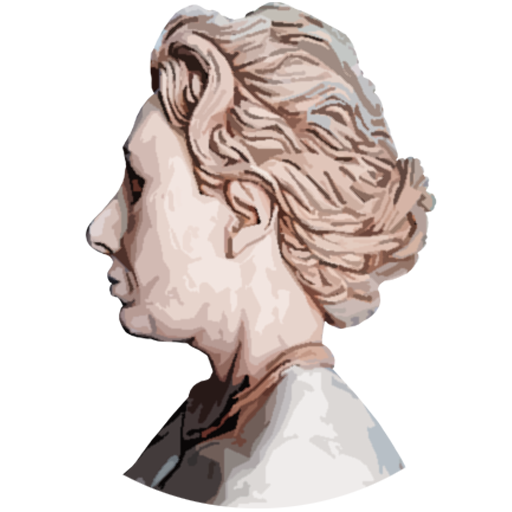
\includegraphics{imagenes/logo.png} 
%\vspace{0.5cm}

{\Huge\bfseries \myTitle \\}
\noindent\rule[-1ex]{\textwidth}{3pt}\\[3.5ex]
{\large\bfseries \mySubtitle \\[4cm]}
\end{minipage}

\vspace{2.5cm}

\noindent\hspace*{\centeroffset}
\begin{minipage}{\textwidth}
\centering
\textbf{Autor}\\ {\myName}\\[2.5ex]
\textbf{Director}\\ {\myProf}\\[2cm]
\end{minipage}

\vspace{\stretch{2}}

\end{titlepage}




\cleardoublepage
\thispagestyle{empty}

\begin{center}
{\large\bfseries \myTitle: \mySubtitle}\\
\end{center}

\begin{center}
\myName \\
\end{center}

\vspace{0.7cm}
\noindent{\textbf{Palabras clave}: palabra\_clave1, palabra\_clave2, palabra\_clave3, ......}\\

\vspace{0.7cm}
\noindent{\textbf{Resumen}}\\

Poner aquí el resumen.

\chapter*{}
\thispagestyle{empty}

\noindent\rule[-1ex]{\textwidth}{2pt}\\[4.5ex]

Yo, \textbf{\myName}, alumno de la titulación \myDegree de la \textbf{\myFaculty}, con DNI 75926571Y, autorizo la ubicación de la siguiente copia de mi Trabajo Fin de Grado en la biblioteca del centro para que pueda ser consultada por las personas que lo deseen.

\vspace{6cm}

\noindent Fdo: \myName

\vspace{2cm}

\begin{flushright}
\myLocation a \myTime.
\end{flushright}


\chapter*{}
\thispagestyle{empty}

\noindent\rule[-1ex]{\textwidth}{2pt}\\[4.5ex]

D. \textbf{\myProf}, Profesor del Área de XXXX del \myDepartment de la \myUni.

\vspace{0.5cm}

\textbf{Informa:}

\vspace{0.5cm}

Que el presente trabajo, titulado \textit{\textbf{\myTitle, \mySubtitle}}, ha sido realizado bajo su supervisión por \textbf{\myName}, y autorizamos la defensa de dicho trabajo ante el tribunal que corresponda.

\vspace{0.5cm}

Y para que conste, expiden y firman el presente informe en \myLocation a \myTime.

\vspace{1cm}

\textbf{El director:}

\vspace{5cm}

\noindent \textbf{\myProf}

\chapter*{Agradecimientos}
\thispagestyle{empty}

\vspace{1cm}

Poner aquí agradecimientos...


\frontmatter
\tableofcontents
\listoffigures
\listoftables
%
\mainmatter
\setlength{\parskip}{5pt}

\chapter{Introducción}
El objetivo de este proyecto es construir un software con el que poder visualizar e interactuar con los datos DICOM obtenidos al someter a una escultura a una Tomografía Axial Computerizada (TAC). 

Para ello se hará uso de VTK, que proporciona una serie de librerías en C++ para facilitar operaciones sobre datos DICOM, y de Qt, para la Interfaz Gráfica de Usuario (GUI).

Antes de empezar con el proyecto en sí, se definirán conceptos como DICOM o TAC que se usarán a lo largo de éste y conviene saber lo que son, así como las distintas herramientas que se utilizarán.

\section{Obtención de datos DICOM mediante un TAC}
DICOM (\textit{Digital Imaging and Comunication in Medicine}) es el estándar internacional para manejar, visualizar, almacenar, imprimir y transmitir imágenes de pruebas médicas (ISO12052) \cite{about_dicom}. 

Al contrario de lo que se puede pensar en un principio, DICOM es más que un formato de imagen, es un protocolo que abarca la transferencia, el almacenamiento y la visualización \cite{dicom_intro_and_guide}.

Pese a que su uso está mayoritariamente extendido en el campo en el que nació (la medicina), se puede usar en otros, como el de la restauración de bienes culturales, como es el caso de este proyecto.

En un archivo DICOM hay almacenado, además de metadatos, una imagen \cite{dicom_classes_vtk} (Figura \ref{fig:prostate_dicom}).

\begin{figure}[H]
	\centering
	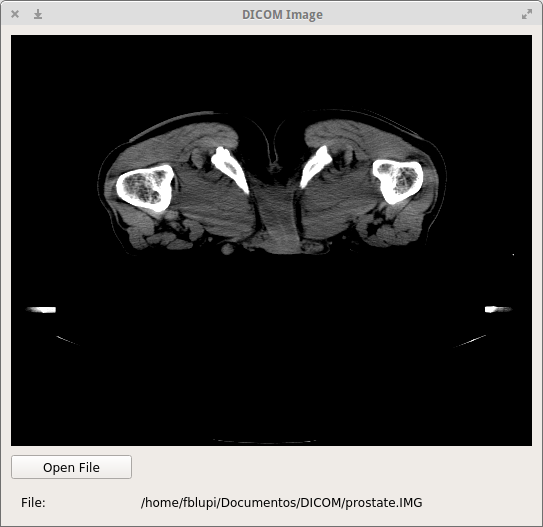
\includegraphics[width=10cm]{imagenes/prostate_dicom}
	\caption{Imagen DICOM de una próstata visualizada con un programa diseñado para visualizar archivos DICOM.}
	\label{fig:prostate_dicom}
\end{figure}

\begin{figure}[H]
	\centering
	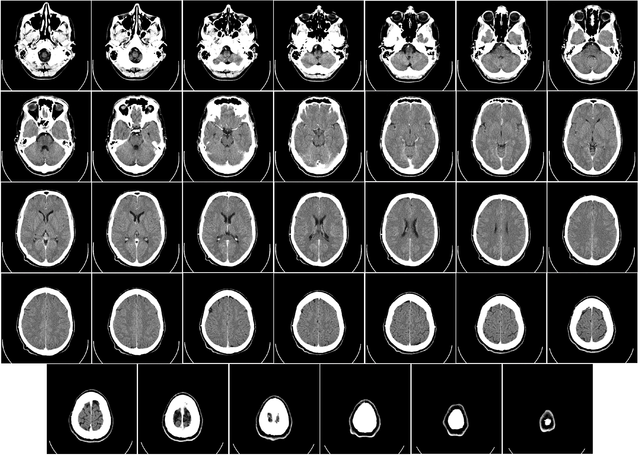
\includegraphics[width=10cm]{imagenes/brain_dicom_serie}
	\caption{Serie de imágenes DICOM extraídas de un TAC realizada a un cerebro.}
	\label{fig:brain_dicom_serie}
\end{figure}

Cuando se realiza un escáner TAC (Tomografía Axial Computerizada) se obtiene una serie de imágenes (Figura \ref{fig:brain_dicom_serie}) de rebanadas del objeto al que se le realiza el escáner. Éstas imágenes se encapsulan en archivos DICOM, y con todas ellas se puede llegar a construir un modelo volumétrico.

El cómo se obtienen las imágenes con un TAC no es objeto de estudio de este proyecto, por lo que no se entrará en mucho detalle. En muy resumidas cuentas, el aparato emite un haz de rayos X desde distintos ángulos al objeto y unos sensores recogen la radiación que absorbe en cada una de estas emisiones. Obteniendo el resultado final del promedio de todas las mediciones que realizan los sensores \cite{tac}. 
\chapter{Especificación de requisitos}

Este capítulo es una Especificación de Requisitos Software para el software que se va a realizar siguiendo las directrices dadas por el estándar IEEE830 \cite{iee830}.

\section{Introducción}

	\subsection{Propósito}
	
	Este capítulo de especificación de requisitos tiene como objetivo definir las especificaciones funcionales y no funcionales para el desarrollo de un software que permitirá visualizar e interactuar con los datos DICOM obtenidos al someter a una escultura a una TC. Éste software será utilizado principalmente por restauradores.
	
	\subsection{Ámbito del sistema}
	
	En la actualidad los datos DICOM obtenidos tras una TC se utilizan, principalmente, en el campo donde surgieron, la medicina. No obstante, esto no significa que solo se pueda aplicar ahí. Con este software, llamado \myTitle, se tratará de trasladar esta técnica al campo de la restauración de bienes culturales y poder visualizar e interactuar con los datos DICOM obtenidos con esculturas.
	
	\subsection{Definiciones, acrónimos y abreviaturas}
	
	\begin{itemize}
		\item \textbf{ERS}: Especificación de Requisitos Software.
		\item \textbf{GUI} (\textit{Graphic User Interface}): Interfaz gráfica de usuario.
		\item \textbf{DICOM} (\textit{Digital Imaging and Comunication in Medicine}): Datos de donde se obtienen las imágenes.
		\item \textbf{TAC o TC} (Tomografía Axial Computerizada): Escáner en el que se obtienen los datos DICOM.
		\item \textbf{GPU} (\textit{Graphic Precessor Unit}): Tarjeta gráfica.
		\item \textbf{VTK} (\textit{The Visualization ToolKit}): Librería gráfica que se utilizará.
		\item \textbf{CMake} (\textit{Cross platform Make}): Herramienta para generar código compilable en distintas plataformas.
		\item \textbf{Qt}: Librería que se utilizará para realizar la GUI.
		\item \textbf{Volumen}: Conjunto de datos en los que para cada posición XYZ se tiene un valor determinado.
		\item \textbf{Corte}: Vista de la figura a través de un plano. Por ejemplo, al cortar con una sierra un tronco por la mitad, se puede ver cómo es por dentro en esa posición por donde se ha cortado.
		\item \textbf{Función de transferencia}: Función utilizada para visualizar los datos deseados de un volumen.
		\item \textbf{\textit{Direct Volume Rendering}}: Visualización directa de volúmenes en la que cada valor del volumen se mapea con un determinado color y opacidad dado por una función de transferencia.
		\item \textbf{\textit{Ray-Casting}}: Técnica de \textit{Direct Volume Rendering} utilizada para la visualización de volúmenes.
		\item \textbf{\textit{Widget}}: Elemento de la GUI.
	\end{itemize}
	
	\subsection{Visión general del documento}
	
	Este capítulo consta de tres secciones:
	\begin{itemize}
		\item En la primera sección se realiza una introducción a éste y se proporciona una visión general de la ERS.
		\item En la segunda sección se realiza una descripción general a alto nivel del software, describiendo los factores que afectan al producto y a sus requisitos y con el objetivo de conocer las principales funcionalidades de éste.
		\item En la tercera sección se definen detalladamente los requisitos que deberá satisfacer el software.
	\end{itemize}

\section{Descripción general}

\subsection{Perspectiva del producto}

	El software \myTitle tiene como objetivo interactuar con datos DICOM, pero no es el encargado de generarlos. Para generarlos se deberá utilizar algún escáner de TC.
	
	Una vez obtenidos, no se necesitará ningún otro software adicional.
	
	\subsection{Funciones del producto}
	
	Las principales funcionalidades de este sistema serán:
	\begin{itemize}
		\item Cargar datos DICOM.
		\item Generar un volumen a partir de los datos cargados.
		\item Visualizar en 3D el volumen.
		\item Modificar la función de transferencia y cambiar colores asignados a cada material.
		\item Generar nuevos cortes.
		\item Visualizar los cortes generados.
		\item Guardar imagen de lo que se visualiza en la pantalla.
	\end{itemize}
	
	\subsection{Características de los usuarios}
	
	Solo existe un tipo de usuario, que es la persona que desee interactuar con los datos DICOM de una escultura. Esta persona no tiene por qué tener habilidad con un equipo informático, por lo que \myTitle deberá tener una GUI intuitiva y fácil de utilizar.
	
	\subsection{Restricciones}
	
	Se llevará a cabo un desarrollo evolutivo basado en un prototipo funcional en el que no están definidos todos los requisitos desde un principio y se irán añadiendo conforme se vayan completando y ocurriendo nuevos.
	
	El software será libre, por lo que el código estará accesible en un repositorio de GitHub.
	
	Se programará en C++ usando las librerías VTK para la visualización de gráficos y Qt para la GUI.
	
	Aprovechando que se debe usar CMake para compilar las librerías mencionadas, se utilizará también para generar el proyecto, pues se puede generar código compilable en distintas plataformas.
	
	\subsection{Suposiciones y dependencias}
	
	El software se utilizará para poder visualizar esculturas de madera por lo que se tendrán en cuenta los materiales con los que están hechas la mayoría de estas. Si se introducen los datos DICOM de cualquier otra cosa con materiales distintos a los utilizados en las esculturas no se visualizará correctamente.

\section{Requisitos específicos}

	\subsection{Interfaces}
	
	La GUI se construirá con Qt y contendrá los siguientes elementos (Figura \ref{fig:basic_gui}):
	\begin{itemize}
		\item \textbf{Barra de menú}: Típica barra de menús (archivo, editar, herramientas...).
		\item \textbf{Barras de herramientas}: Acceso rápido con los botones de las operaciones más utilizadas sobre cada \textit{widget} de visualización.
		\item \textbf{\textit{Widget} de visualización del volumen en 3D}: Con el que se podrá interactuar para girar, hacer zoom y ver la figura desde distintas posiciones.
		\item \textbf{\textit{Widget} de visualización de cortes}: En el que se mostrará el corte que se genera con un plano determinado.
		\item \textbf{Menú de operaciones}: Menú organizado en pestañas donde se podrán realizar distintas operaciones como cambiar la función de transferencia y definir el plano para realizar un corte.
	\end{itemize}
	
	\begin{figure}[H]
		\centering
		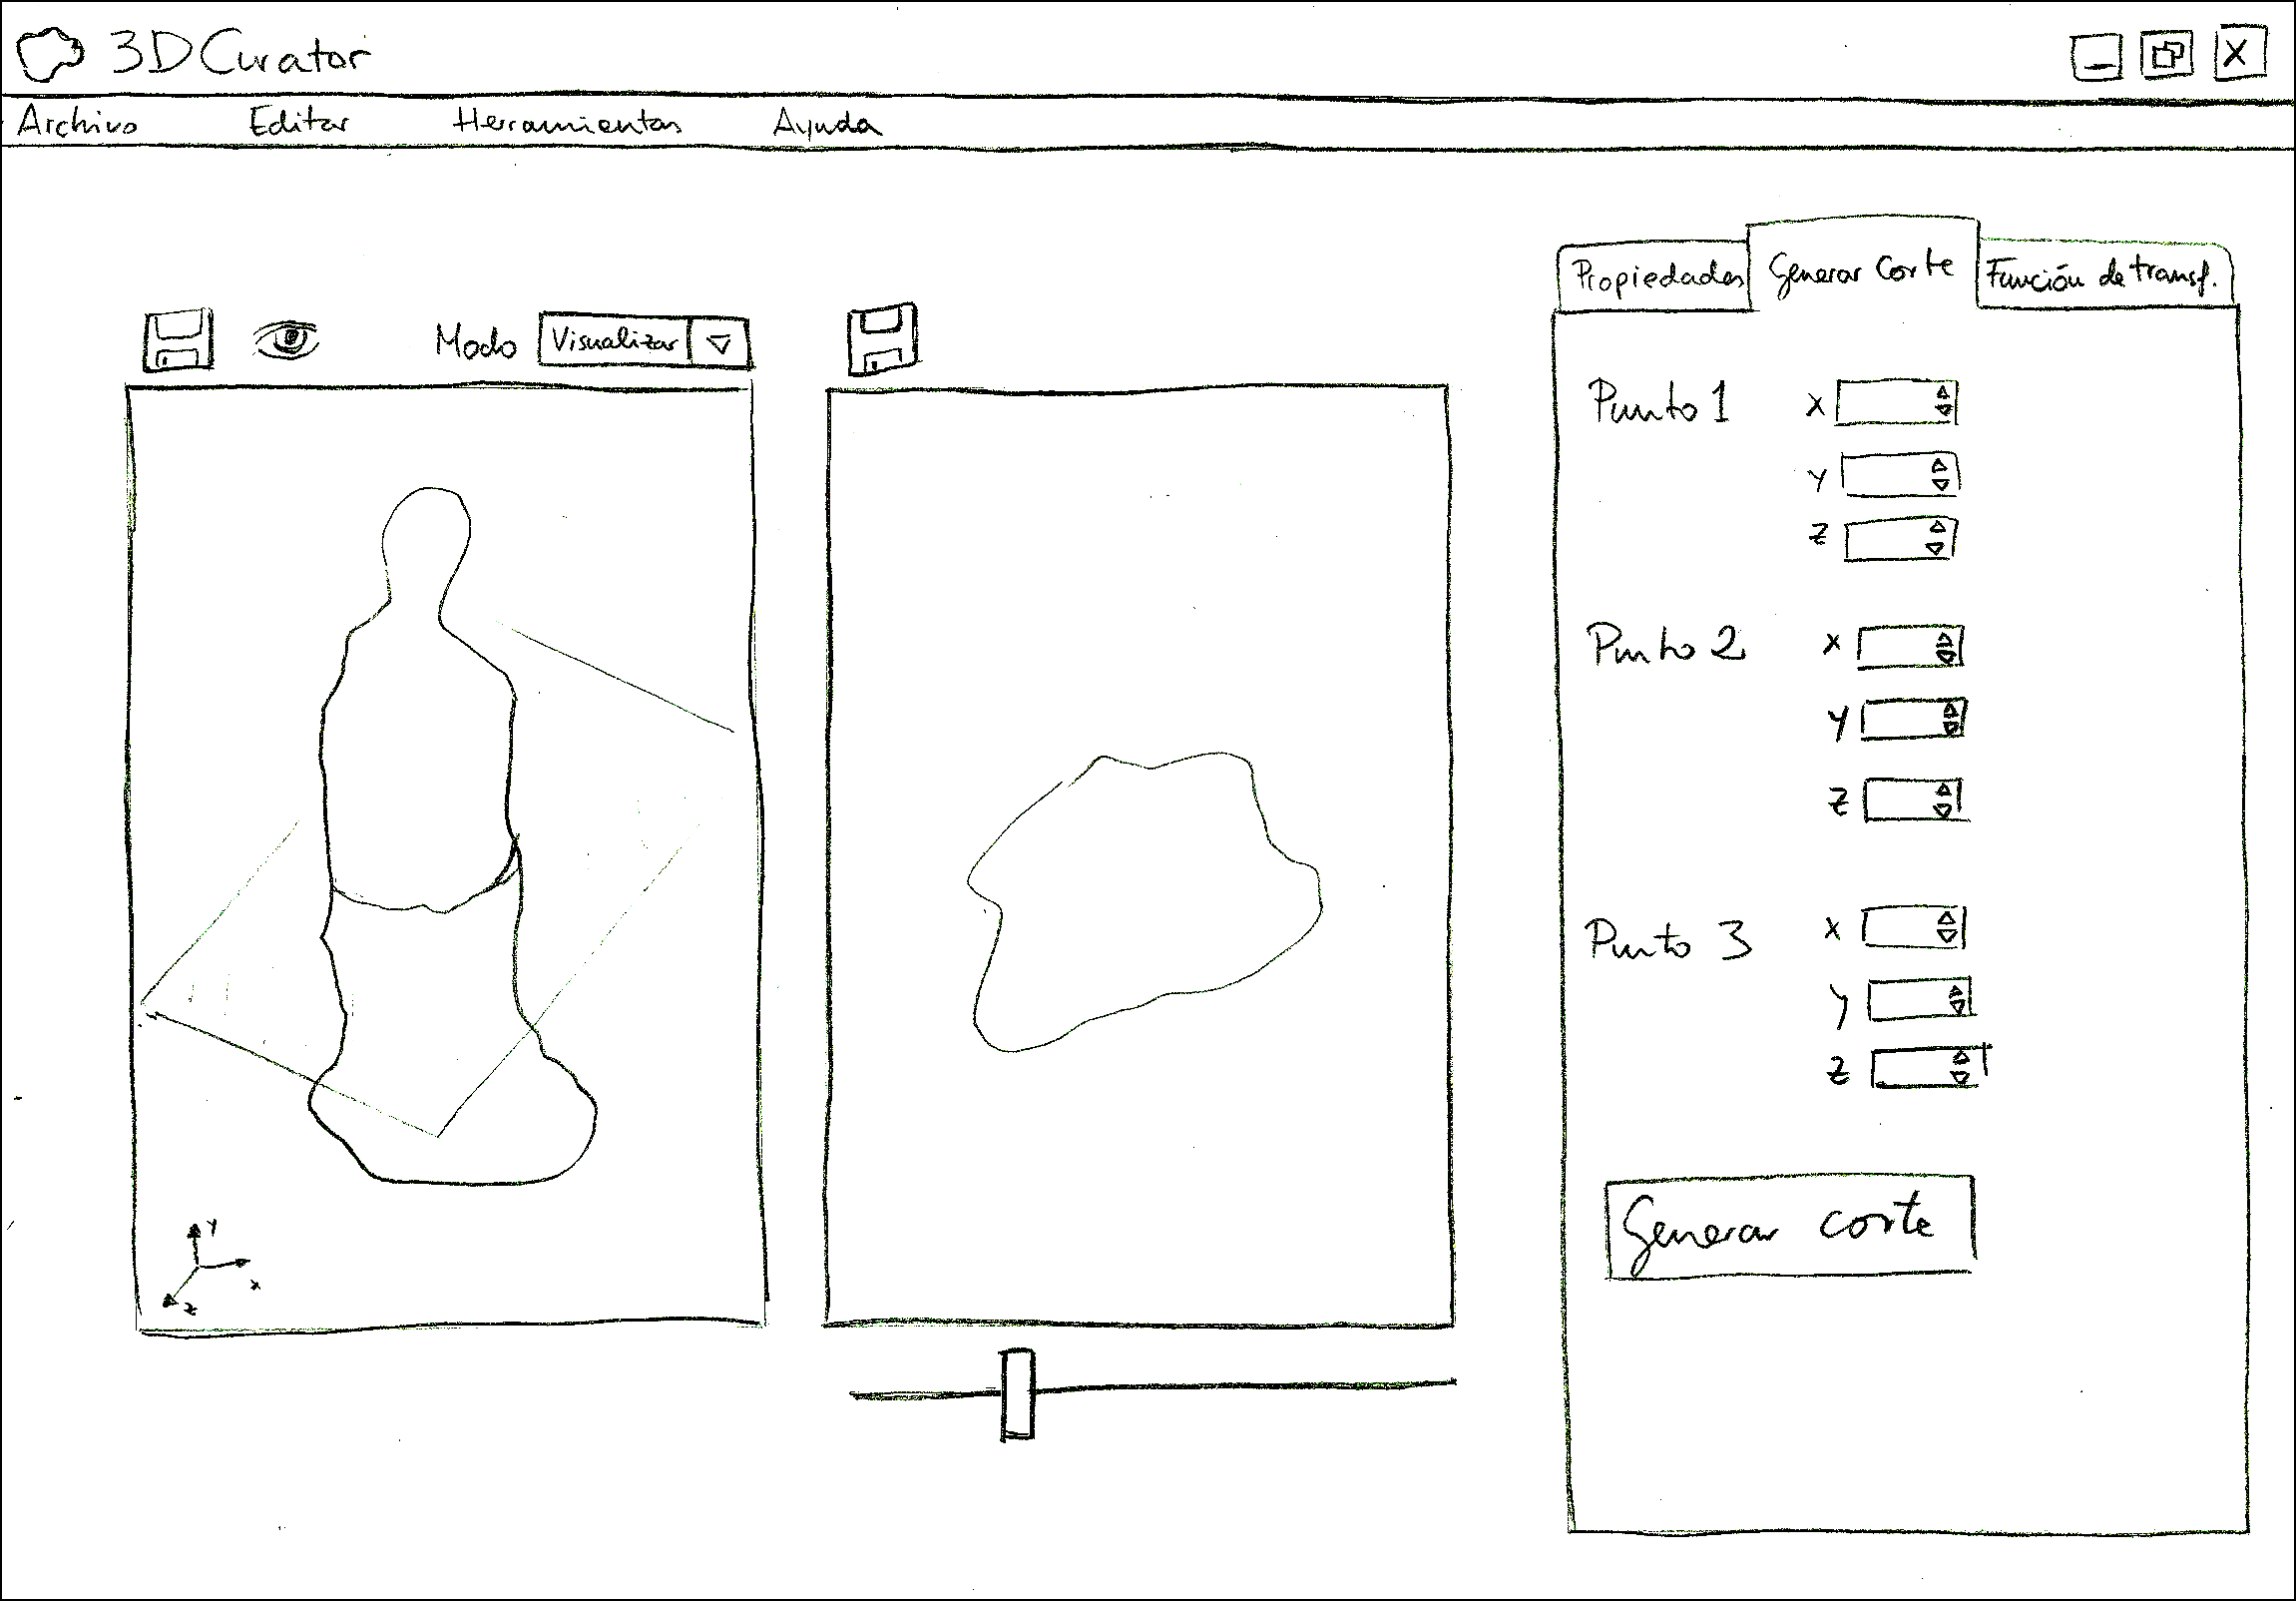
\includegraphics[width=12.5cm]{imagenes/basic_gui}
		\caption{Boceto a mano alzada de la posible distribución de los elementos en la GUI}
		\label{fig:basic_gui}
	\end{figure}
	
	\subsection{Funciones}
	
	El sistema tendrá que realizar distintas funciones que se comentaron anteriormente pero se profundizará en esta sección. Se han estructurado estas funciones por su objetivo separando cuatro subsecciones distintas: Lectura de datos, generación de cortes, visualización y configuración.
	
		\subsubsection{Lectura de datos}
		\begin{itemize}
			\item \textbf{Seleccionar carpeta}: Cuando el usuario quiera cargar datos DICOM, le aparecerá una ventana donde se podrá escoger alguna carpeta de su sistema de forma que solo muestre las carpetas y no los archivos.
			\item \textbf{Verificar que la carpeta contiene datos DICOM}: Se tendrá que verificar que el usuario ha seleccionado una carpeta con datos DICOM y se le avisará si no lo ha hecho.
			\item \textbf{Cargar datos DICOM}: Cuando se haya seleccionado una carpeta correcta, se cargarán los datos y automáticamente los visualizará en 3D con la configuración por defecto.
		\end{itemize}
	
		\subsubsection{Generación de cortes}
		\begin{itemize}
			\item \textbf{Definir plano}: El usuario podrá definir un plano por donde realizar un corte a la figura. Para ello tendrá que introducir tres puntos. Por defecto, se introducirá un plano en el eje XZ a una altura de Y = 0, siendo la dirección de los ejes XYZ la que utiliza VTK (Figura \ref{fig:vtk_axes}). El plano se podrá visualizar en el \textit{widget} de visualización 3D para ver gráficamente por dónde pasará.
			\begin{figure}[H]
				\centering
				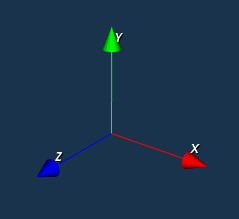
\includegraphics[width=8cm]{imagenes/vtk_axes}
				\caption{Dirección de los ejes XYZ}
				\label{fig:vtk_axes}
			\end{figure}
			\item \textbf{Modificar plano}: El usuario podrá modificar el plano o introduciendo nuevos puntos, o interactuando con la vista previa de éste en el \textit{widget} de visualización 3D. Las operaciones que podrá realizar en este serán:
			\begin{itemize}
				\item Rotar en cualquiera de los ejes.
				\item Trasladar en dirección de la normal.
			\end{itemize}
			\item \textbf{Generar corte}: Una vez se haya creado el plano deseado, se podrá mostrar el corte en el \textit{widget} de visualización de cortes.
		\end{itemize}
	
		\subsubsection{Visualización}
		\begin{itemize}
			\item \textbf{Visualizar en 3D}: Cuando el usuario haya seleccionado una carpeta con datos DICOM, se mostrará en 3D en el \textit{widget} izquierdo pudiendo rotar y hacer zoom interactuando con el ratón. Para visualizar el volumen se utilizarán técnicas de \textit{Direct Volume Rendering} que proporcionan VTK como puede ser el \textit{Ray-Casting}.
			\item \textbf{Visualizar corte}: Cuando el usuario haya cargado los datos DICOM y haya establecido un plano de corte, se podrá generar un corte a la figura por éste. Este corte se visualizará en el \textit{widget} derecho.
			\item \textbf{Guardar imagen}: El usuario en todo momento podrá guardar una imagen (en formatos comunes JPG o PNG) de lo que está viendo en cada uno de los \textit{widgets} seleccionando en una ventana que aparecerá cuando se elija la opción la dirección donde se guardará y el nombre del archivo. 
		\end{itemize}
	
		\subsubsection{Configuración}
		\begin{itemize}
			\item \textbf{Cambiar color de fondo}: El usuario podrá cambiar el color de fondo del \textit{widget} donde se mostrará la figura en 3D. Para ello podrá:
			\begin{itemize}
				\item Elegir entre colores predeterminados.
				\item Introducir un color mediante valores RGB.
				\item Introducir un color mediante su código de color hexadecimal.
			\end{itemize}
			\item \textbf{Cambiar función de transferencia}: El usuario podrá cambiar la función de transferencia utilizada para poder ver los distintos materiales con una paleta de color distinta a la que se da por defecto.
		\end{itemize}
	
	\subsection{Requisitos de rendimiento}
	
	Al ser una aplicación de escritorio donde no se almacenarán datos sino que se mostrarán, los requisitos de rendimiento no se centrarán en la concurrencia de acceso ni en el almacenamiento, como lo podrían estar en una aplicación web.
	
	Sin embargo, hay que tener en cuenta otros factores, como pueden ser el uso eficiente de memoria y no tener cargadas todas las figuras que se han estado visualizando, desechando la anterior cuando se carga una nueva.
	
	El rendimiento gráfico también es importante, por eso y para obtener imágenes de mayor calidad, se utilizarán técnicas de \textit{Direct Volume Rendering} como el \textit{Ray-Casting}. Estas técnicas necesitan una gran cantidad de procesamiento, pero la velocidad de procesamiento de las GPUs actuales no deberían resultar un problema.
	
	\subsection{Restricciones de diseño}
	
	Al utilizar la librería VTK se seguirá su estructura a la hora de construir el software, y se tendrán restricciones en cuanto a funcionalidad que se pueda construir con ésta. No obstante es una librería muy completa y no se debería encontrar ninguna restricción viendo otros programas de visualización de datos médicos que se han construido usando esta librería.
	
	\subsection{Atributos del software}
	
	Al usar CMake, se podrá crear un software multiplataforma que funcione en cualquier sistema operativo.
	
	El software generado deberá ser fiable, porque aunque no trabaje con datos sensibles cuya pérdida pueda ser grave, siempre resulta molesto utilizar un software con fallos que interrumpan durante su uso.
	
	También se debe tener en cuenta que el software sea mantenible pues, al ser libre, otros desarrolladores pueden colaborar en su desarrollo y debe estar bien documentado para que esto sea una tarea fácil.
\chapter{Especificación de requisitos}

En este capítulo comentaré la planificación inicial de tiempo en la que se llevará a cabo este TFG y la estimación de horas para cada tarea.

\section{Fechas y aclaraciones}

La primera reunión con mi tutor fue el día \textbf{11 de Noviembre}, así que se puede dar esa fecha como fecha de inicio. La fecha de entrega, en este momento en el que se realiza la planificación, es desconocida. Pero espero tener el software terminado para la última semana de Mayo o primera de Junio, por lo que he puesto como fecha de fin el \textbf{9 de Junio}.

Al llevarse a cabo un desarrollo evolutivo incremental, no están concretados todos los requisitos que satisfará el software, por lo que solo están definidos los requisitos iniciales, aunque si se han planificado horas para las posteriores mejoras. Estos requisitos se descompondrán en tareas una vez se definan y se irán acoplando al espacio temporal reservado.

Al hacerse esta planificación tras la segunda reunión, todas las tareas tanto de la primera como de la segunda no tienen el número de horas estimadas, sino las empleadas realmente.

La estimación para cada tarea ha sido difícil de asignar por ser la primera vez que voy a trabajar con VTK y Qt, pero espero que la experiencia que he adquirido en las prácticas que he realizado en las distintas asignaturas que he tenido durante estos cuatro años me ayude y logre hacer una buena planificación.

\section{Planificación}

He troceado el calendario con un \textit{sprint} de reunión en reunión (cada dos semanas) y el resultado ha sido el siguiente:

\begin{itemize}
	\item \textbf{Reunión 1} (13/11/15 - 26/11/15)
	\begin{itemize}
		\item Instalación de entorno de desarrollo (12 horas)
		\item Aprender VTK (4 horas)
		\item Aprender Qt (3 horas)
		\item Aprender estructura DICOM (3 horas)
	\end{itemize}
	
	\item \textbf{Reunión 2} (27/11/15 - 10/12/15)
	\begin{itemize}
		\item Especificación de requisitos (6 horas)
		\item Planificación (2 horas)
		\item Visualización de volumen básica (10 horas)
	\end{itemize}
	
	\item \textbf{Reunión 3} (11/12/15 - 7/1/16)
	\begin{itemize}
		\item Interacción con la cámara (8 horas)
		\item Estudiar función de transferencia (12 horas)
		\item Implementar función de transferencia (12 horas)
		\item Escribir en la memoria (4 horas)
	\end{itemize}
	
	\item \textbf{Reunión 4} (8/1/16 - 21/1/16)
	\begin{itemize}
		\item Modificar función de transferencia (15 horas)
		\item Visualizar plano (5 horas)
	\end{itemize}
	
	\item \textbf{Reunión 5} (22/1/16 - 4/2/16)
	\begin{itemize}
		\item Modificar plano dando puntos (5 horas)
		\item Modificar plano interactuando con éste (15 horas)
	\end{itemize}
	
	\item \textbf{Reunión 6} (5/2/16 - 18/2/16)
	\begin{itemize}
		\item Generar corte con el plano (8 horas)
		\item Visualizar corte generado (12 horas)
	\end{itemize}
	
	\item \textbf{Reunión 7} (19/2/16 - 3/3/16)
	\begin{itemize}
		\item Interactuar con cortes generados (6 horas)
		\item Guardar imágenes (8 horas)
		\item Testeos intensivos (4 horas)
		\item Corrección de \textit{bugs} (6 horas)
		\item Escribir en la memoria (4 horas)
	\end{itemize}
	
	\item \textbf{Reunión 8} (4/3/16 - 17/3/16)
	\begin{itemize}
		\item Mejora \#1 (18 horas)
		\item Escribir en la memoria (2 horas)
	\end{itemize}
	
	\item \textbf{Reunión 9} (18/3/16 - 31/3/16)
	\begin{itemize}
		\item Mejora \#2 (18 horas)
		\item Escribir en la memoria (2 horas)
	\end{itemize}
	
	\item \textbf{Reunión 10} (1/4/16 - 14/4/16)
	\begin{itemize}
		\item Mejora \#3 (18 horas)
		\item Escribir en la memoria (2 horas)
	\end{itemize}
	
	\item \textbf{Reunión 11} (15/4/16 - 28/4/16)
	\begin{itemize}
		\item Mejora \#4 (18 horas)
		\item Escribir en la memoria (2 horas)
	\end{itemize}
	
	\item \textbf{Reunión 12} (29/4/16 - 12/5/16)
	\begin{itemize}
		\item Mejora \#5 (18 horas)
		\item Escribir en la memoria (2 horas)
	\end{itemize}
	
	\item \textbf{Reunión 13} (13/5/16 - 26/5/16)
	\begin{itemize}
		\item Mejora \#6 (18 horas)
		\item Escribir en la memoria (2 horas)
	\end{itemize}
	
	\item \textbf{Reunión 14} (27/5/16 - 9/6/16)
	\begin{itemize}
		\item Revisar y terminar la memoria (6 horas)
		\item Preparar la exposición (10 horas)
	\end{itemize}
\end{itemize}

En total se estima que se realicen unas \textbf{300 horas}. Se llevará a cabo un recuento de horas realizadas para ver, finalmente, cuántas se han necesitado.
\chapter{Análisis}

\section{Técnicas de renderizado}

A la hora de renderizar un conjunto de datos volumétricos para obtener una imagen en 3D, se pueden utilizar distintas técnicas y VTK proporciona una serie de clases para su uso:
\begin{itemize}
	\item \textbf{\textit{Marching Cubes}}: Con este algoritmo se obtiene una malla poligonal de una isosuperficie a partir de un conjunto de datos volumétrico (Figura \ref{fig:marching_cubes_head}) \cite{marching_cubes}. Se puede usar en VTK con \texttt{vtkMarchingCubes}.
	\begin{figure}[H]
		\centering
		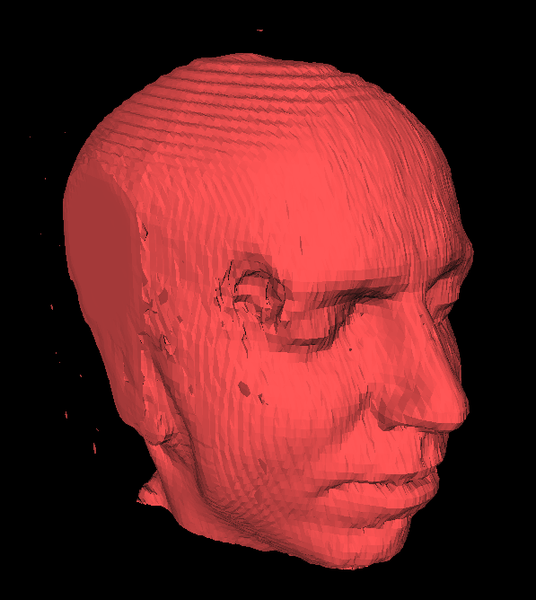
\includegraphics[width=6cm]{imagenes/marching_cubes_head}
		\caption{Cabeza extraída de 150 cortes obtenidos por una IRM usando \textit{marching cubes} (sobre 150.000 triángulos). Imagen extraída de \url{https://en.wikipedia.org/wiki/File:Marchingcubes-head.png}}
		\label{fig:marching_cubes_head}
	\end{figure}
	
	\item \textbf{Texturas 2D}: Se utilizan planos de corte alineados a los ejes de coordenadas. Por lo que se tendría una serie de cortes sobre el plano sagital, otra sobre el coronal y otra sobre el axial. Se realiza una interpolación bilineal para obtener la imagen final (Figura \ref{fig:texturas2d} \cite{intro_medical_vtk_bioimage}). Se puede usar en VTK con \texttt{vtkVolumeTextureMapper}.
	\begin{figure}[H]
		\centering
		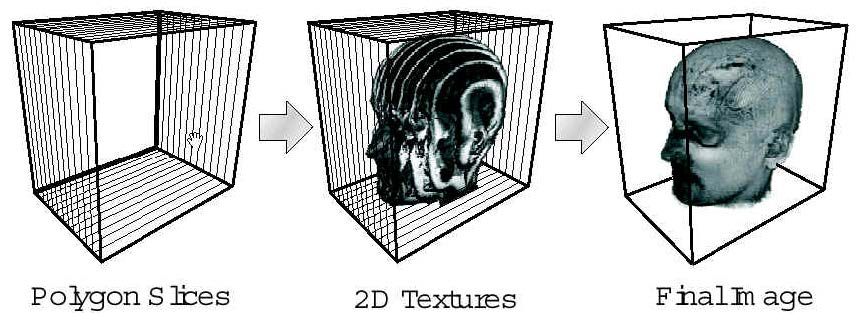
\includegraphics[width=10cm]{imagenes/texturas2d}
		\caption{Esquema del proceso de renderizado usando texturas 2D. Imagen extraída del apéndice B del libro \textit{An Introduction to Programming for Medical Image Analysis with the Visualization Toolkit }\cite{intro_medical_vtk_bioimage}}
		\label{fig:texturas2d}
	\end{figure}
	
	\item \textbf{Texturas 3D}: Esta técnica es similar a la anterior, pero ahora los datos se cargan en una textura 3D y los cortes se dibujan paralelos a la dirección de vista. A diferencia de las texturas 2D, usa interpolación trilineal y no es necesario tener almacenado en memoria tres copias de los mismos datos (Figura \ref{fig:texturas3d}) \cite{intro_medical_vtk_bioimage}. Se puede usar en VTK con \texttt{vtkVolumeTextureMapper3D}.
	\begin{figure}[H]
		\centering
		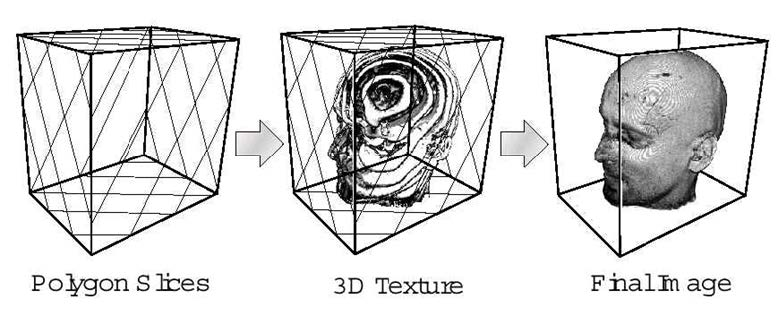
\includegraphics[width=10cm]{imagenes/texturas3d}
		\caption{Esquema del proceso de renderizado usando texturas 3D. Imagen extraída del apéndice B del libro \textit{An Introduction to Programming for Medical Image Analysis with the Visualization Toolkit} \cite{intro_medical_vtk_bioimage}}
		\label{fig:texturas3d}
	\end{figure}
	
	\item \textbf{\textit{Volume Ray Casting}}: Es una técnica en el que para cada pixel de la imagen se lanza un rayo que atraviesa el volumen. Para cada voxel se obtiene su color y opacidad usando una función de transferencia. Cuando el rayo sale del volumen se calcula el color y opacidad del pixel como el acumulado por el rayo. Existe una versión de este algoritmo que hace uso de la GPU para acelerar ostensiblemente el tiempo de la operación (Figura \ref{fig:volume_ray_casting}) \cite{intro_medical_vtk_bioimage}. Se puede usar en VTK con \texttt{vtkFixedVolumeRayCastMapper}, \texttt{vtkVolumeRayCastMapper} (usan CPU), \texttt{vtkGPUVolumeRayCastMapper} (usa GPU) y \texttt{vtkSmartVolumeMapper} (según el contexto usa CPU o GPU).
	\begin{figure}[H]
		\centering
		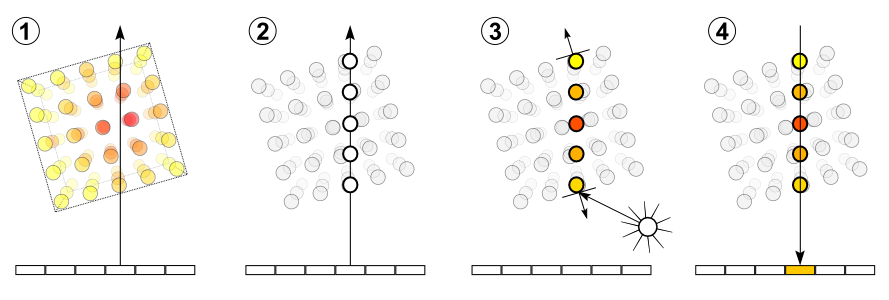
\includegraphics[width=12.5cm]{imagenes/volume_ray_casting}
		\caption{Esquema del proceso de \textit{ray casting}. Imagen extraída de \url{https://en.wikipedia.org/wiki/File:Volume_ray_casting.png}}
		\label{fig:volume_ray_casting}
	\end{figure}
\end{itemize}

De entre todas estas técnicas, se podrían descartar rápidamente la de \textit{marching cubes}: pues tan solo trabaja con isosuperficies y la de texturas 2D: pues la opción de texturas 3D es más rápida y usa menos recursos.

Por tanto ya solo habría que elegir entre texturas 3D o \textit{ray casting}. Hasta hace unos años, VTK no proporcionaba un algoritmo de \textit{ray casting} que usase la GPU. Por tanto la opción habría sido sencilla, pero durante los últimos años han trabajado en esto haciendo del \textit{ray casting} la opción preferible.

\section{Volume Mapper}

Para poder visualizar un volumen con VTK mediante Direct Volume Rendering (DVR), necesitamos un \textit{Volume Mapper}. La librería nos ofrece varias alternativas:
\begin{itemize}
	\item \texttt{vtkAMRVolumeMapper}
	\item \texttt{vtkFixedVolumeRayCastMapper}
	\item \texttt{vtkGPUVolumeRayCastMapper}
	\item \texttt{vtkSmartVolumeMapper}
	\item \texttt{vtkVolumeRayCastMapper}
	\item \texttt{vtkVolumeTextureMapper}
	\item \texttt{vtkVolumeTextureMapper3D}
\end{itemize}

Entre esta lista tenemos algunos que utilizan o texturas o \textit{ray casting}, o la CPU o la GPU. Pero hay uno que es especial con respecto al resto. Se trata de \texttt{vtkSmartVolumeMapper}.

Este \textit{Volume Mapper} es una versión mejorada del \texttt{vtkGPUVolumeRayCast Mapper} por lo que utiliza la GPU (si el dispositivo cuenta con una) y la técnica de \textit{ray casting}. Además cuenta con nuevas características con respecto al resto, como el poder definir infinitos planos de corte para poder ver el interior del volumen \cite{smart_volume_mapper}.

Por tanto, el \textit{Volume Mapper} utilizado será el \texttt{vtkSmartVolumeMapper}.

\section{Función de transferencia}

La función de transferencia es la encargada de dar a un valor de intensidad las propiedades de color y opacidad que le corresponden para la visualización del volumen.

En VTK la función de transferencia forma parte de la clase \texttt{vtkVolume Property} \cite{vtk_example_medical4}. Para ello proporciona otras dos clases:
\begin{itemize}
	\item \texttt{vtkColorTransferFunction}: Para definir el color. Se enlaza a \texttt{vtk VolumeProperty} con el método \texttt{SetColor}.
	\item \texttt{vtkPiecewiseFunction}: Para definir la opacidad (tanto escalar como gradiente). La opacidad escalar se enlaza a \texttt{vtkVolumeProperty} con el método \texttt{SetScalarOpacity} y la gradiente con \texttt{SetGradientOpacity}.
\end{itemize}

Podemos, por tanto, diferenciar tres partes fundamentales en la función de transferencia, la encargada de dar la propiedad de color y las dos de dar la propiedad de opacidad. Ambas trabajan de forma independiente. Es decir, cuando se define un punto en una de ellas, no tiene por qué definirse en la otra.

\subsection{Color}

Para definir esta función (\texttt{vtkColorTransferFunction}), hay que agregar puntos para valores de intensidad a los que se les asignará un color. VTK se encargará de interpolar entre un punto y otro (Figura \ref{fig:color_tf}). 

Por defecto, cuando no hay ningún punto, a todos los valores de intensidad les corresponderá un color negro. De forma parecida se comporta cuando solo hay un punto pero en lugar de negro, les corresponderá el color del punto que se ha definido.

VTK permite trabajar tanto con HSV como con RGB y para añadir un punto hay que utilizar \texttt{AddHSVPoint} o \texttt{AddRGBPoint}. A estos métodos se les pasa un primer parámetro en coma flotante con el valor de intensidad donde se establecerá ese punto y otros tres con las distintas exponentes (\textit{hue}, \textit{saturation}, \textit{brightness} o \textit{red}, \textit{green}, \textit{blue}).

\begin{figure}[H]
	\centering
	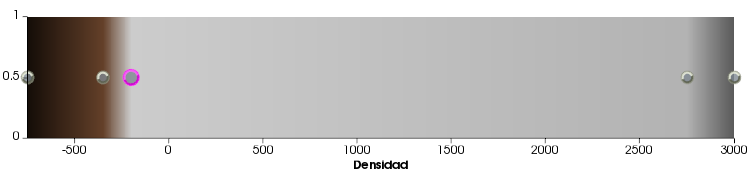
\includegraphics[width=12.5cm]{imagenes/color_tf}
	\caption{Parte de color de la función de transferencia del \textit{preset} \textit{CT-WoodSculpture} creado para visualizar esculturas de madera policromadas. Dos puntos definen el color. Uno en -750 con un tono más oscuro y otro en -350 con un tono más claro. El estuco se pinta con un color gris claro y también viene definido por dos puntos: -200 y 2750. Finalmente, el metal se verá con un tono gris oscuro definido con un punto en 3000.}
	\label{fig:color_tf}
\end{figure}

\subsection{Opacidad}

El valor de opacidad se obtendría como el \textbf{producto de la opacidad escalar por la gradiente}. Si no se define alguna de las dos, se definiría como un valor constante de 1 para que solo se viese el resultado de la que sí está definida.

\subsubsection{Opacidad escalar}

Con el color no bastaría, pues si comprobásemos ahora añadiéndole tan solo el \texttt{vtkColorTransferFunction} al \texttt{vtkVolumeProperty} observaríamos que no se pinta nada en pantalla. Esto es porque por defecto, al no tener ningún punto la función de opacidad (\texttt{vtkPiecewiseFunction}) es una constante con valor 0 (transparente). 

Para definir esta función se trabaja de forma parecida a como se hace con el color, añadiendo puntos. El método que hay que utilizar es \texttt{AddPoint} al que se le pasan dos parámetros en coma flotante. El primero con el valor de intensidad y el segundo con la opacidad en ese punto. Para obtener los valores en puntos intermedios, se interpola entre los dos puntos en los que está. De forma que si para el valor de intensidad 100 hemos definido una opacidad de 0.5 y para el de 200 1, al valor de intensidad 150 le corresponderá 0.75.

Combinando color y opacidad escalar podemos obtener una función de transferencia para visualizar nuestro volumen (Figura \ref{fig:opacity_tf}), pero para obtener mejores resultados, habrá que utilizar la opacidad gradiente. 

\begin{figure}[H]
	\centering
	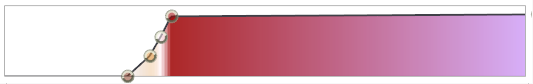
\includegraphics[width=12.5cm]{imagenes/opacity_tf}
	\caption{Parte de opacidad escalar de la función de transferencia del \textit{preset} \textit{CT-WoodSculpture} creado para visualizar esculturas de madera policromadas. Se pueden observar tres regiones. La primera corresponde a la madera, la segunda al estuco y la última al metal}
	\label{fig:opacity_tf}
\end{figure}

\subsubsection{Opacidad gradiente}

La opacidad gradiente utiliza el vector gradiente para dar el valor de opacidad. Con éste se puede conseguir \textbf{dar un mayor valor a regiones de los bordes, así como menor a regiones planas} es decir, donde no varía el valor de intensidad de sus vecinos de alrededor.

El gradiente se mide como la cantidad que varía la intensidad en una unidad de distancia. Este cálculo del gradiente lo realiza VTK cuando genera el volumen de forma transparente sin que haya que añadir nada al código.

Para poder definir la función de la opacidad gradiente, al igual que con las demás, hay que añadir puntos con la misma función que se usaba con la opacidad escalar (\texttt{AddPoint}). 

\begin{figure}[H]
	\centering
	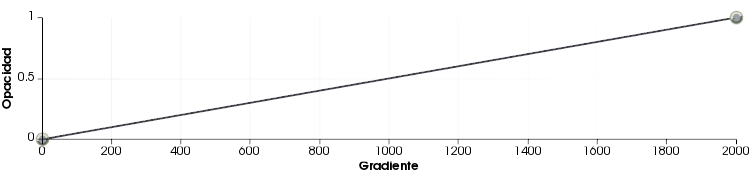
\includegraphics[width=12.5cm]{imagenes/gradient_tf}
	\caption{Parte de opacidad gradiente de la función de transferencia del \textit{preset} \textit{CT-WoodSculpture} creado para visualizar esculturas de madera policromadas. Se obtendría un valor cercano a 1 en la opacidad en aquellas zonas más cercanas a los bordes entre materiales pues se ha establecido que para un gradiente 0 la opacidad sea 0, y para 2000, 1. }
	\label{fig:gradient_tf}
\end{figure}

\section{Escala Hounsfield}

Como ya se ha explicado, para desarrollar la función de transferencia con la que se visualiza el volumen, juega un papel muy importante el valor de densidad del material. 

Este valor se encuentra en unas unidades conocidas como Unidades Hounsfield (HU) en honor al ingeniero Godfrey Newbold Hounsfield, inventor del primer escáner TAC con el que ganó el Premio Nobel de Fisiología o Medicina en 1979.

La Escala Hounsfield no es más que la transformación de la escala de coeficientes de atenuación lineal de rayos X a una nueva en relación al valor del agua destilada en condiciones normales de presión y temperatura.

El valor de HU de un material viene dado por la siguiente fórmula:

\[ HU = 1000 \times \frac{\mu_{mat}-\mu_{agua}}{\mu_{agua}} \]

Donde $ \mu_{mat} $ es el coeficiente de atenuación lineal del material y $ \mu_{agua} $ el del agua.

Por tanto, el valor teórico del agua será 0 HU.

El rango de valores de la escala va desde -1024 HU hasta 3071 HU. 4096 valores representados mediante 12 bits.

\begin{table}[H]
	\begin{center}
		\begin{tabular} {|l|l|}
			\hline
			Material & HU \\ \hline
			\hline
			Aire & -1000 \\ \hline
			Madera & -750 a -350 \\ \hline
			Estuco & 200 a 1000 \\ \hline
			Metal & 2900 a 3000 \\ \hline
		\end{tabular}
		\caption{Valores en HU de distintos materiales presentes en imágenes de esculturas de madera}
		\label{tab:materials_hu}
	\end{center}
\end{table}

\section{Historias de usuario}

% Explicar que se han ido añadiendo poco a poco

\begin{table}[H]
	\begin{center}
		\begin{tabular} {|l|c|l|}
			\hline
			1 & \multicolumn{2}{c|}{Cargar datos DICOM} \\ \hline \hline
			\multicolumn{3}{|l|}{Descripción} \\ \hline
			\multicolumn{3}{|p{12cm}|}{Se debe dotar al software de funcionalidad para cargar datos DICOM de un directorio. Para ello el usuario explorará entre los directorios del sistema hasta encontrar aquel con los datos que se desean visualizar.} \\ \hline
			\multicolumn{2}{|l|}{Estimación} & 1 \\ \hline
			\multicolumn{2}{|l|}{Prioridad} & 1 \\ \hline
			\multicolumn{2}{|l|}{Dependencias} & - \\ \hline
			\multicolumn{3}{|l|}{Pruebas de aceptación} \\ \hline
			\multicolumn{3}{|p{12cm}|}{ - Se selecciona un directorio sin datos DICOM o mal formateados y se informa del fallo.} \\ 
			\multicolumn{3}{|p{12cm}|}{ - Se selecciona un directorio con datos DICOM y se cargan correctamente.} \\ \hline
		\end{tabular}
	\end{center}
	\caption{Historia de usuario - Cargar datos DICOM}
	\label{tab:hu_cargar_datos_dicom}
\end{table}

\begin{table}[H]
	\begin{center}
		\begin{tabular} {|l|c|l|}
			\hline
			2 & \multicolumn{2}{c|}{Generar reconstrucción 3D} \\ \hline \hline
			\multicolumn{3}{|l|}{Descripción} \\ \hline
			\multicolumn{3}{|p{12cm}|}{A partir de un directorio con datos DICOM se almacenan en un volumen que se renderiza en 3D usando ray casting en una ventana.} \\ \hline
			\multicolumn{2}{|l|}{Estimación} & 4 \\ \hline
			\multicolumn{2}{|l|}{Prioridad} & 1 \\ \hline
			\multicolumn{2}{|l|}{Dependencias} & - \\ \hline
			\multicolumn{3}{|l|}{Pruebas de aceptación} \\ \hline
			\multicolumn{3}{|p{12cm}|}{ - A partir de unos datos DICOM se genera y se visualiza correctamente el volumen.} \\ \hline
		\end{tabular}
	\end{center}
	\caption{Historia de usuario - Generar reconstrucción 3D}
	\label{tab:hu_generar_reconstruccion_3d}
\end{table}

\begin{table}[H]
	\begin{center}
		\begin{tabular} {|l|c|l|}
			\hline
			3 & \multicolumn{2}{c|}{Cambiar material de la figura} \\ \hline \hline
			\multicolumn{3}{|l|}{Descripción} \\ \hline
			\multicolumn{3}{|p{12cm}|}{El usuario podrá cambiar el material con el que se visualiza la figura cambiando sus componentes ambiental, difuso, especular y potencia especular introduciendo un valor entre 0 a 1 en los tres primeros y uno entre 1 y 50 en el último.} \\ \hline
			\multicolumn{2}{|l|}{Estimación} & 2 \\ \hline
			\multicolumn{2}{|l|}{Prioridad} & 4 \\ \hline
			\multicolumn{2}{|l|}{Dependencias} & - \\ \hline
			\multicolumn{3}{|l|}{Pruebas de aceptación} \\ \hline
			\multicolumn{3}{|p{12cm}|}{ - El usuario no puede introducir un valor en ninguna de las componentes fuera del rango de valores.} \\
			\multicolumn{3}{|p{12cm}|}{ - Cuando se cambia el material la figura pasa a visualizarse con este.} \\ \hline
		\end{tabular}
	\end{center}
	\caption{Historia de usuario - Cambiar material de la figura}
	\label{tab:hu_cambiar_material_de_la_figura}
\end{table}

\begin{table}[H]
	\begin{center}
		\begin{tabular} {|l|c|l|}
			\hline
			4 & \multicolumn{2}{c|}{Cambiar color de fondo} \\ \hline \hline
			\multicolumn{3}{|l|}{Descripción} \\ \hline
			\multicolumn{3}{|p{12cm}|}{El usuario podrá cambiar el color de fondo de cada uno de las ventanas en cualquiera de sus modos.} \\ \hline
			\multicolumn{2}{|l|}{Estimación} & 2 \\ \hline
			\multicolumn{2}{|l|}{Prioridad} & 4 \\ \hline
			\multicolumn{2}{|l|}{Dependencias} & - \\ \hline
			\multicolumn{3}{|l|}{Pruebas de aceptación} \\ \hline
			\multicolumn{3}{|p{12cm}|}{ - El usuario no puede introducir un color incorrecto.} \\
			\multicolumn{3}{|p{12cm}|}{ - Cuando el usuario cambia los colores de las ventanas, estas se actualizan con su nuevo color de fondo.} \\ \hline
		\end{tabular}
	\end{center}
	\caption{Historia de usuario - Cambiar color de fondo}
	\label{tab:hu_cambiar_color_de_fondo}
\end{table}

\begin{table}[H]
	\begin{center}
		\begin{tabular} {|l|c|l|}
			\hline
			5 & \multicolumn{2}{c|}{Generar y visualizar cortes} \\ \hline \hline
			\multicolumn{3}{|l|}{Descripción} \\ \hline
			\multicolumn{3}{|p{12cm}|}{A partir de la reconstrucción 3D del volumen y un plano que se podrá mover y girar arbitrariamente, se visualizará el corte que produce este plano con el volumen en una ventana distinta a la utilizada para visualizarlo en 3D.} \\ \hline
			\multicolumn{2}{|l|}{Estimación} & 6 \\ \hline
			\multicolumn{2}{|l|}{Prioridad} & 1 \\ \hline
			\multicolumn{2}{|l|}{Dependencias} & 2 \\ \hline
			\multicolumn{3}{|l|}{Pruebas de aceptación} \\ \hline
			\multicolumn{3}{|p{12cm}|}{ - Cuando no hay ningún volumen cargado no se visualiza nada en la ventana de cortes.} \\ 
			\multicolumn{3}{|p{12cm}|}{ - Cuando hay un volumen el plano solo se puede mover a través de este.} \\ 
			\multicolumn{3}{|p{12cm}|}{ - Cuando el plano interseca con el volumen se visualiza correctamente el corte.} \\ \hline
		\end{tabular}
	\end{center}
	\caption{Historia de usuario - Generar y visualizar cortes}
	\label{tab:hu_generar_y_visualizar_cortes}
\end{table}

\begin{table}[H]
	\begin{center}
		\begin{tabular} {|l|c|l|}
			\hline
			6 & \multicolumn{2}{c|}{Cambiar plano de corte} \\ \hline \hline
			\multicolumn{3}{|l|}{Descripción} \\ \hline
			\multicolumn{3}{|p{12cm}|}{A partir del plano de corte en cualquier posición, se podrá girar en cualquiera de los ejes y mover a través de la dirección de su normal.} \\ \hline
			\multicolumn{2}{|l|}{Estimación} & 3 \\ \hline
			\multicolumn{2}{|l|}{Prioridad} & 1 \\ \hline
			\multicolumn{2}{|l|}{Dependencias} & 5 \\ \hline
			\multicolumn{3}{|l|}{Pruebas de aceptación} \\ \hline
			\multicolumn{3}{|p{12cm}|}{ - Cuando se realiza la transformación en el plano, se actualiza la imagen del corte que produce en la figura.} \\ \hline
		\end{tabular}
	\end{center}
	\caption{Historia de usuario - Cambiar plano de corte}
	\label{tab:hu_cambiar_plano_de_corte}
\end{table}

\begin{table}[H]
	\begin{center}
		\begin{tabular} {|l|c|l|}
			\hline
			7 & \multicolumn{2}{c|}{Habilitar y deshabilitar el plano de corte} \\ \hline \hline
			\multicolumn{3}{|l|}{Descripción} \\ \hline
			\multicolumn{3}{|p{12cm}|}{El usuario podrá habilitar y deshabilitar el plano de corte para visualizarlo o no en el visor 3D.} \\ \hline
			\multicolumn{2}{|l|}{Estimación} & 2 \\ \hline
			\multicolumn{2}{|l|}{Prioridad} & 1 \\ \hline
			\multicolumn{2}{|l|}{Dependencias} & 5 \\ \hline
			\multicolumn{3}{|l|}{Pruebas de aceptación} \\ \hline
			\multicolumn{3}{|p{12cm}|}{ - Cuando el plano está habilitado y se ejecuta la acción, este se deshabilita.} \\
			\multicolumn{3}{|p{12cm}|}{ - Cuando el plano está deshabilitado y se ejecuta la acción, este se habilita.} \\ \hline
		\end{tabular}
	\end{center}
	\caption{Historia de usuario - Habilitar y deshabilitar el plano de corte}
	\label{tab:hu_habilitar_y_deshabilitar_el_plano_de_corte}
\end{table}

\begin{table}[H]
	\begin{center}
		\begin{tabular} {|l|c|l|}
			\hline
			8 & \multicolumn{2}{c|}{Posiciones por defecto del plano} \\ \hline \hline
			\multicolumn{3}{|l|}{Descripción} \\ \hline
			\multicolumn{3}{|p{12cm}|}{Se puede colocar el plano directamente en el centro del volumen en posiciones axial, sagital y coronal.} \\ \hline
			\multicolumn{2}{|l|}{Estimación} & 3 \\ \hline
			\multicolumn{2}{|l|}{Prioridad} & 3 \\ \hline
			\multicolumn{2}{|l|}{Dependencias} & 5 \\ \hline
			\multicolumn{3}{|l|}{Pruebas de aceptación} \\ \hline
			\multicolumn{3}{|p{12cm}|}{ - El plano se coloca en la posición deseada cuando se realiza la acción.} \\ \hline
		\end{tabular}
	\end{center}
	\caption{Historia de usuario - Posiciones por defecto del plano}
	\label{tab:hu_posiciones_por_defecto_del_plano}
\end{table}

\begin{table}[H]
	\begin{center}
		\begin{tabular} {|l|c|l|}
			\hline
			9 & \multicolumn{2}{c|}{Guardar imágenes de las ventanas} \\ \hline \hline
			\multicolumn{3}{|l|}{Descripción} \\ \hline
			\multicolumn{3}{|p{12cm}|}{Se podrán guardar imágenes de lo que se visualiza en las ventanas tanto en formato JPG como PNG. Para ello el usuario eligirá dónde almacenar la imagen generada. Por defecto el nombre para la imagen corresponderá con la fecha como cadena de números en formato "AAAAMMDDHHMMSS".} \\ \hline
			\multicolumn{2}{|l|}{Estimación} & 2 \\ \hline
			\multicolumn{2}{|l|}{Prioridad} & 2 \\ \hline
			\multicolumn{2}{|l|}{Dependencias} & - \\ \hline
			\multicolumn{3}{|l|}{Pruebas de aceptación} \\ \hline
			\multicolumn{3}{|p{12cm}|}{ - Si el usuario guarda sin escribir la extensión, comprobar que se añade automáticamente.} \\
			\multicolumn{3}{|p{12cm}|}{ - Si el usuario guarda con un nombre y una extensión, comprobar que efectivamente ocurre así.} \\ \hline
		\end{tabular}
	\end{center}
	\caption{Historia de usuario - Guardar imágenes de las ventanas}
	\label{tab:hu_guardar_imagenes_de_las_ventanas}
\end{table}

\begin{table}[H]
	\begin{center}
		\begin{tabular} {|l|c|l|}
			\hline
			10 & \multicolumn{2}{c|}{Cambiar función de transferencia} \\ \hline \hline
			\multicolumn{3}{|l|}{Descripción} \\ \hline
			\multicolumn{3}{|p{12cm}|}{Se podrá cambiar la función de transferencia con la que visualizar el volumen eligiendo entre varios presets que se presentan.} \\ \hline
			\multicolumn{2}{|l|}{Estimación} & 3 \\ \hline
			\multicolumn{2}{|l|}{Prioridad} & 2 \\ \hline
			\multicolumn{2}{|l|}{Dependencias} & - \\ \hline
			\multicolumn{3}{|l|}{Pruebas de aceptación} \\ \hline
			\multicolumn{3}{|p{12cm}|}{ - Si el usuario cambia la función de transferencia, se actualiza la visualización del volumen usando esta.} \\ \hline
		\end{tabular}
	\end{center}
	\caption{Historia de usuario - Cambiar función de transferencia}
	\label{tab:hu_cambiar_funcion_de_transferencia}
\end{table}

\begin{table}[H]
	\begin{center}
		\begin{tabular} {|l|c|l|}
			\hline
			11 & \multicolumn{2}{c|}{Editar función de transferencia} \\ \hline \hline
			\multicolumn{3}{|l|}{Descripción} \\ \hline
			\multicolumn{3}{|p{12cm}|}{El usuario podrá editar la función de transferencia, para ello se le proporcionará un gráfico con cada una de las partes (color, opacidad escalar y gradiente) que podrá modificar añadiendo, quitando y moviendo puntos.} \\ \hline
			\multicolumn{2}{|l|}{Estimación} & 8 \\ \hline
			\multicolumn{2}{|l|}{Prioridad} & 3 \\ \hline
			\multicolumn{2}{|l|}{Dependencias} & - \\ \hline
			\multicolumn{3}{|l|}{Pruebas de aceptación} \\ \hline
			\multicolumn{3}{|p{12cm}|}{ - Si el usuario intenta borrar un punto cuando solo quedan dos, no se le dejará.} \\
			\multicolumn{3}{|p{12cm}|}{ - Si se edita cualquiera de las partes de la función de transferencia se cambia esta y, por tanto, la visualización del volumen.} \\ \hline
		\end{tabular}
	\end{center}
	\caption{Historia de usuario - Editar función de transferencia}
	\label{tab:hu_editar_funcion_de_transferencia}
\end{table}

\begin{table}[H]
	\begin{center}
		\begin{tabular} {|l|c|l|}
			\hline
			12 & \multicolumn{2}{c|}{Exportar función de transferencia} \\ \hline \hline
			\multicolumn{3}{|l|}{Descripción} \\ \hline
			\multicolumn{3}{|p{12cm}|}{Se podrá exportar la función de transferencia actual a un archivo XML.} \\ \hline
			\multicolumn{2}{|l|}{Estimación} & 5 \\ \hline
			\multicolumn{2}{|l|}{Prioridad} & 4 \\ \hline
			\multicolumn{2}{|l|}{Dependencias} & - \\ \hline
			\multicolumn{3}{|l|}{Pruebas de aceptación} \\ \hline
			\multicolumn{3}{|p{12cm}|}{ - Si el usuario guarda sin escribir la extensión, comprobar que se añade automáticamente.} \\
			\multicolumn{3}{|p{12cm}|}{ - Si el usuario guarda con un nombre, comprobar que efectivamente ocurre así.} \\ \hline
		\end{tabular}
	\end{center}
	\caption{Historia de usuario - Exportar función de transferencia}
	\label{tab:hu_exportar_funcion_de_transferencia}
\end{table}

\begin{table}[H]
	\begin{center}
		\begin{tabular} {|l|c|l|}
			\hline
			13 & \multicolumn{2}{c|}{Importar función de transferencia} \\ \hline \hline
			\multicolumn{3}{|l|}{Descripción} \\ \hline
			\multicolumn{3}{|p{12cm}|}{El usuario podrá importar una función de transferencia almacenada en un archivo XML con un formato determinado.} \\ \hline
			\multicolumn{2}{|l|}{Estimación} & 6 \\ \hline
			\multicolumn{2}{|l|}{Prioridad} & 4 \\ \hline
			\multicolumn{2}{|l|}{Dependencias} & - \\ \hline
			\multicolumn{3}{|l|}{Pruebas de aceptación} \\ \hline
			\multicolumn{3}{|p{12cm}|}{ - Si el usuario carga un archivo XML con un formato distinto al usado para exportar funciones de transferencia, se informará del error.} \\
			\multicolumn{3}{|p{12cm}|}{ - Si el usuario introduce un archivo correcto, se carga la función de transferencia.} \\ \hline
		\end{tabular}
	\end{center}
	\caption{Historia de usuario - Importar función de transferencia}
	\label{tab:hu_importar_funcion_de_transferencia}
\end{table}

\begin{table}[H]
	\begin{center}
		\begin{tabular} {|l|c|l|}
			\hline
			14 & \multicolumn{2}{c|}{Realizar medidas} \\ \hline \hline
			\multicolumn{3}{|l|}{Descripción} \\ \hline
			\multicolumn{3}{|p{12cm}|}{El usuario podrá realizar varias medidas de un punto a otro en cualquiera de las dos ventanas.} \\ \hline
			\multicolumn{2}{|l|}{Estimación} & 6 \\ \hline
			\multicolumn{2}{|l|}{Prioridad} & 2 \\ \hline
			\multicolumn{2}{|l|}{Dependencias} & - \\ \hline
			\multicolumn{3}{|l|}{Pruebas de aceptación} \\ \hline
			\multicolumn{3}{|p{12cm}|}{ - Si el usuario introduce dos puntos se visualiza una línea de uno a otro con la medida correspondiente.} \\ \hline
		\end{tabular}
	\end{center}
	\caption{Historia de usuario - Realizar medida}
	\label{tab:hu_realizar_medida}
\end{table}

\begin{table}[H]
	\begin{center}
		\begin{tabular} {|l|c|l|}
			\hline
			15 & \multicolumn{2}{c|}{Añadir regla} \\ \hline \hline
			\multicolumn{3}{|l|}{Descripción} \\ \hline
			\multicolumn{3}{|p{12cm}|}{El usuario podrá añadir reglas para realizar medidas en cualquiera de las dos ventanas.} \\ \hline
			\multicolumn{2}{|l|}{Estimación} & 3 \\ \hline
			\multicolumn{2}{|l|}{Prioridad} & 2 \\ \hline
			\multicolumn{2}{|l|}{Dependencias} & 14 \\ \hline
			\multicolumn{3}{|l|}{Pruebas de aceptación} \\ \hline
			\multicolumn{3}{|p{12cm}|}{ - Si el usuario añade una regla en una ventana, se puede realizar la medida en esta.} \\
			\multicolumn{3}{|p{12cm}|}{ - Si el usuario intenta añadir más reglas que las establecidas por un límite, se le informa y no se añade.} \\ \hline
		\end{tabular}
	\end{center}
	\caption{Historia de usuario - Añadir regla}
	\label{tab:hu_anadir_regla}
\end{table}

\begin{table}[H]
	\begin{center}
		\begin{tabular} {|l|c|l|}
			\hline
			16 & \multicolumn{2}{c|}{Eliminar regla} \\ \hline \hline
			\multicolumn{3}{|l|}{Descripción} \\ \hline
			\multicolumn{3}{|p{12cm}|}{El usuario podrá eliminar cualquier regla creada con anterioridad.} \\ \hline
			\multicolumn{2}{|l|}{Estimación} & 3 \\ \hline
			\multicolumn{2}{|l|}{Prioridad} & 2 \\ \hline
			\multicolumn{2}{|l|}{Dependencias} & 14 \\ \hline
			\multicolumn{3}{|l|}{Pruebas de aceptación} \\ \hline
			\multicolumn{3}{|p{12cm}|}{ - Si el usuario elimina una regla, se elimina correctamente y deja de visualizarse.} \\
			\multicolumn{3}{|p{12cm}|}{ - Si el usuario intenta eliminar cuando no hay ninguna regla, se le informa de esto.} \\ \hline
		\end{tabular}
	\end{center}
	\caption{Historia de usuario - Eliminar regla}
	\label{tab:hu_eliminar_regla}
\end{table}

\begin{table}[H]
	\begin{center}
		\begin{tabular} {|l|c|l|}
			\hline
			17 & \multicolumn{2}{c|}{Habilitar y deshabilitar regla} \\ \hline \hline
			\multicolumn{3}{|l|}{Descripción} \\ \hline
			\multicolumn{3}{|p{12cm}|}{El usuario podrá habilitar o deshabilitar una regla para mostrarla o no sin llegar a borrarla.} \\ \hline
			\multicolumn{2}{|l|}{Estimación} & 2 \\ \hline
			\multicolumn{2}{|l|}{Prioridad} & 3 \\ \hline
			\multicolumn{2}{|l|}{Dependencias} & 14 \\ \hline
			\multicolumn{3}{|l|}{Pruebas de aceptación} \\ \hline
			\multicolumn{3}{|p{12cm}|}{ - Si el usuario deshabilita una regla habilitada, deja de mostrarse.} \\
			\multicolumn{3}{|p{12cm}|}{ - Si el usuario habilita una regla deshabilitada, se vuelve a mostrar.} \\
			\multicolumn{3}{|p{12cm}|}{ - Si el usuario intenta eliminar cuando no hay ninguna regla, se le informa de esto.} \\ \hline
		\end{tabular}
	\end{center}
	\caption{Historia de usuario - Habilitar y deshabilitar regla}
	\label{tab:hu_habilitar_y_deshabilitar_regla}
\end{table}

\begin{table}[H]
	\begin{center}
		\begin{tabular} {|l|c|l|}
			\hline
			18 & \multicolumn{2}{c|}{Eliminar partes} \\ \hline \hline
			\multicolumn{3}{|l|}{Descripción} \\ \hline
			\multicolumn{3}{|p{12cm}|}{El usuario podrá eliminar una parte del volumen separada de las demás seleccionando un punto de esta.} \\ \hline
			\multicolumn{2}{|l|}{Estimación} & 10 \\ \hline
			\multicolumn{2}{|l|}{Prioridad} & 2 \\ \hline
			\multicolumn{2}{|l|}{Dependencias} & - \\ \hline
			\multicolumn{3}{|l|}{Pruebas de aceptación} \\ \hline
			\multicolumn{3}{|p{12cm}|}{ - Si el usuario selecciona un punto se elimina la parte seleccionada.} \\ \hline
		\end{tabular}
	\end{center}
	\caption{Historia de usuario - Eliminar partes}
	\label{tab:hu_eliminar_partes}
\end{table}
\chapter{Diseño}

\section{Diagramas de clases}

\subsection{Paquete Application}

\begin{figure}[H]
	\centering
	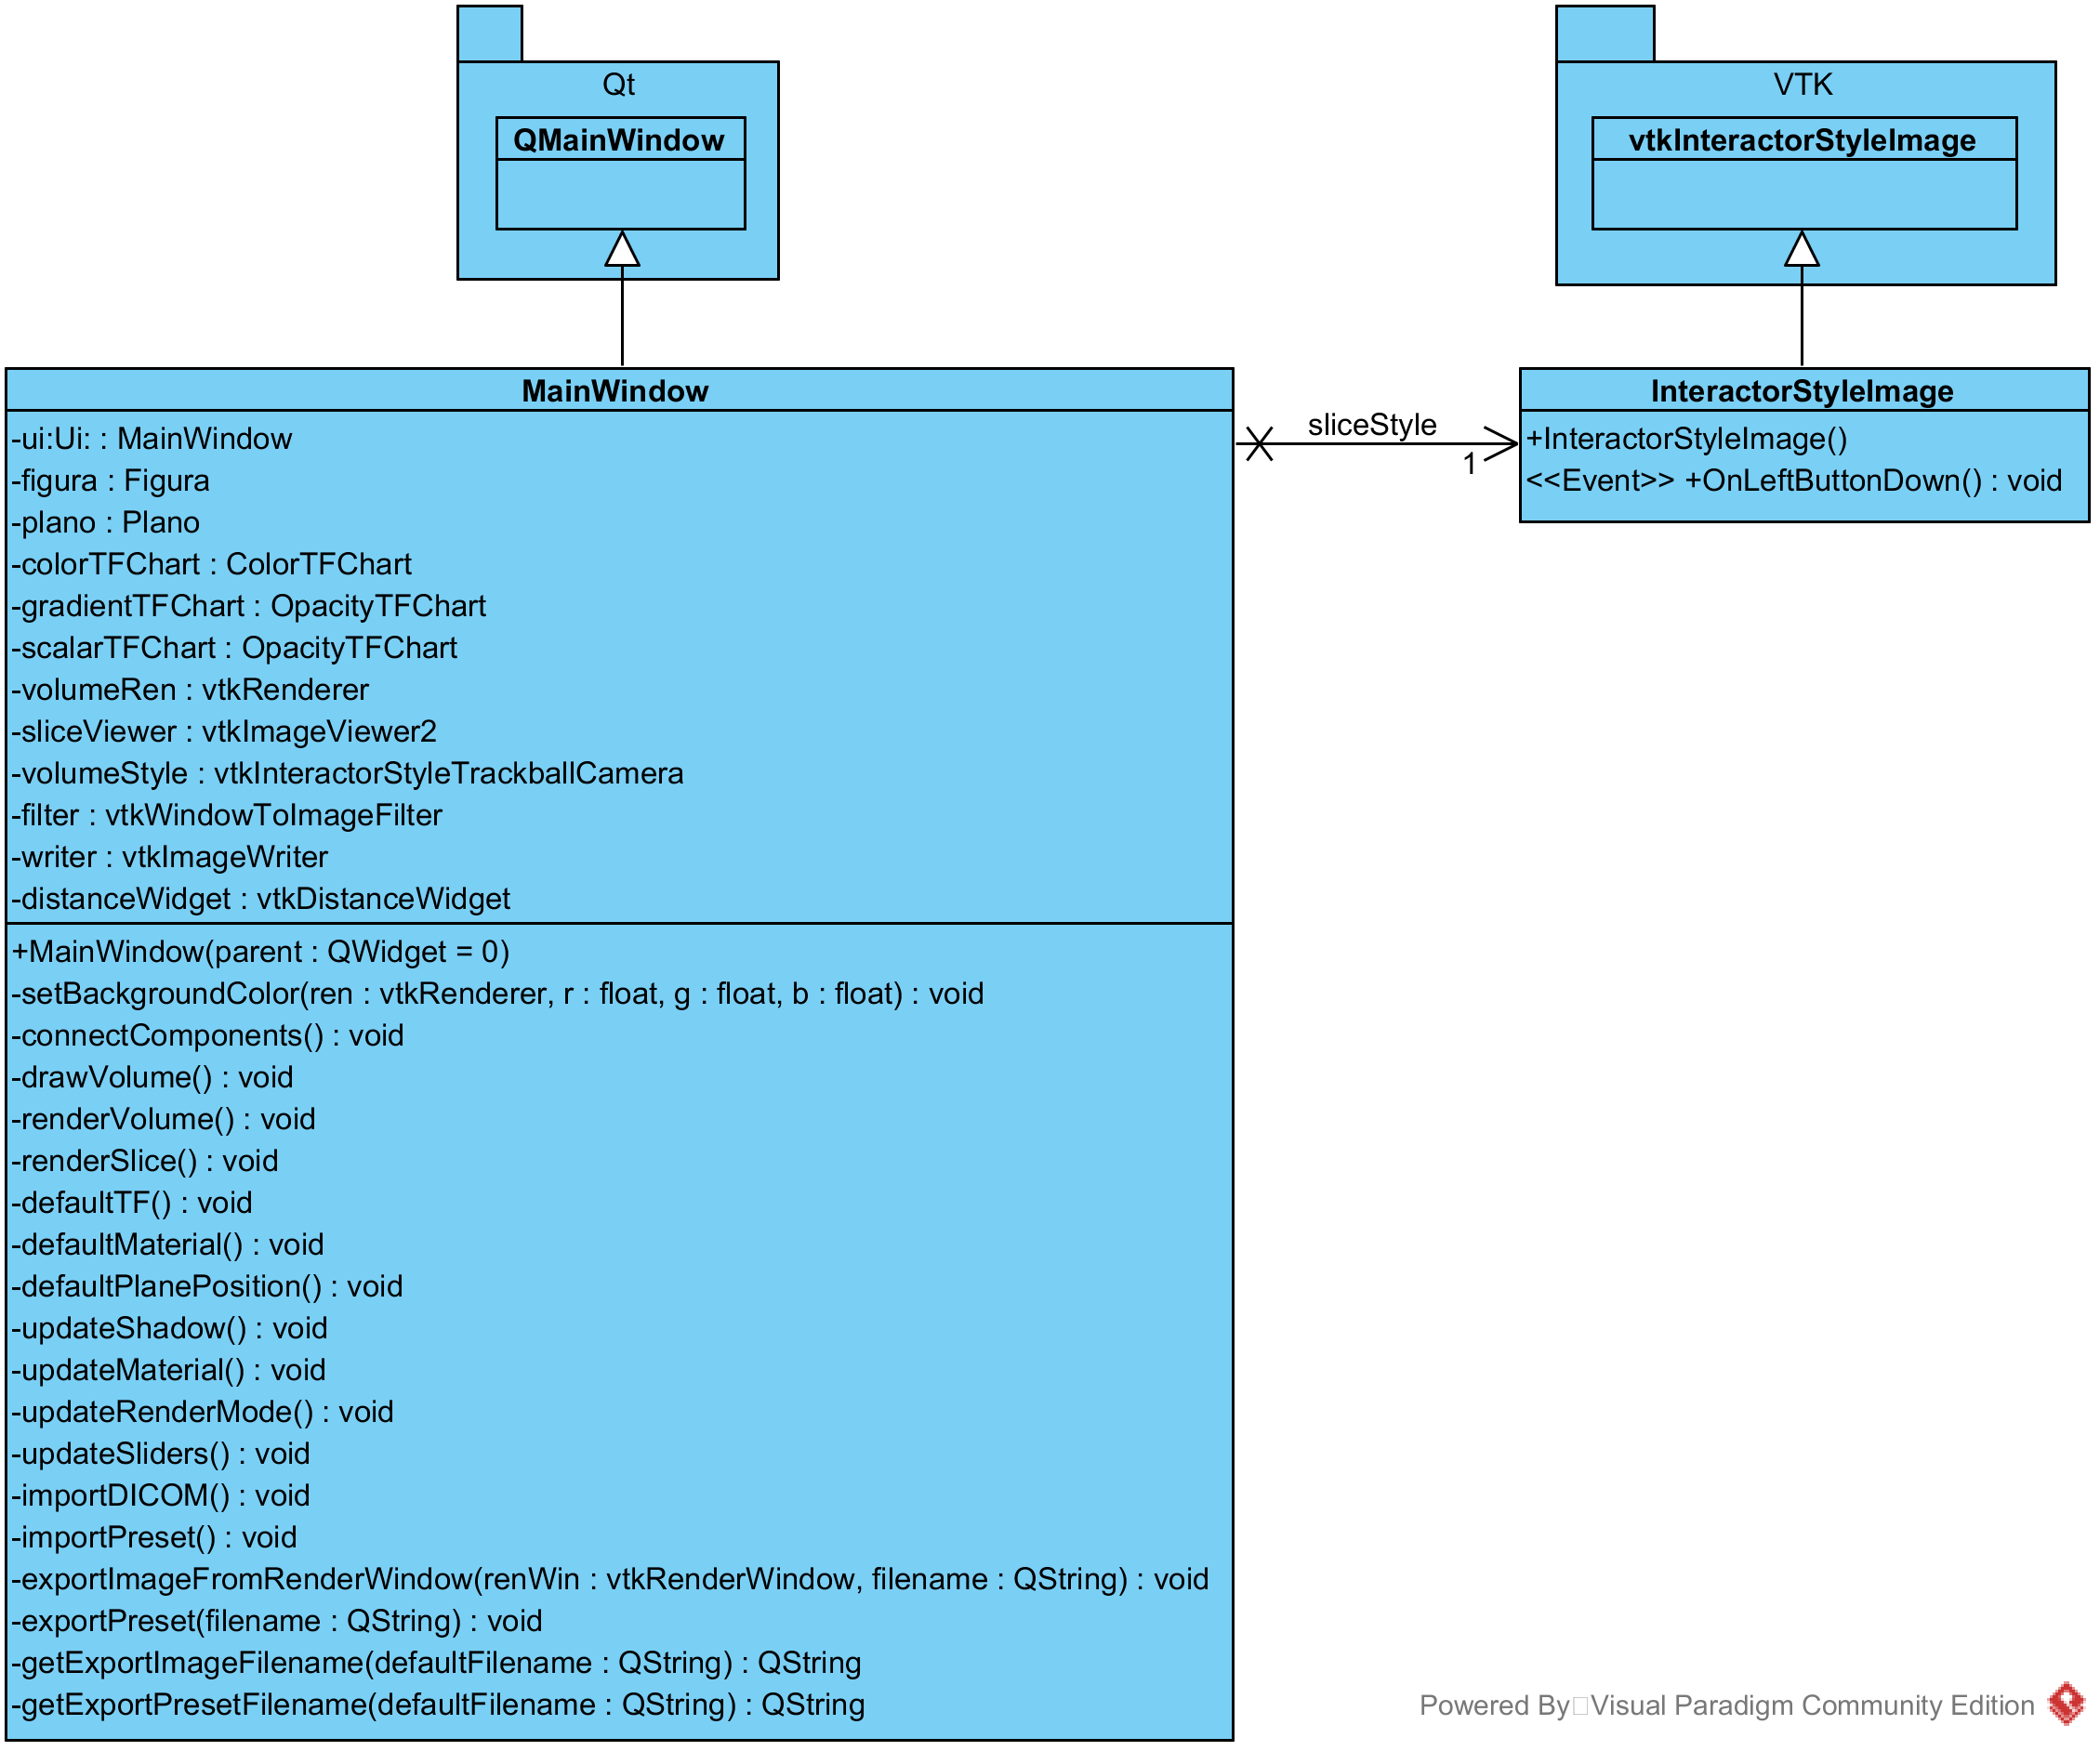
\includegraphics[width=12.5cm]{imagenes/diagramas/application}
	\caption{Diagrama de clases del paquete \textit{Application}}
	\label{fig:diagrama_clases_application}
\end{figure}

\subsection{Paquete Charts}

\begin{figure}[H]
	\centering
	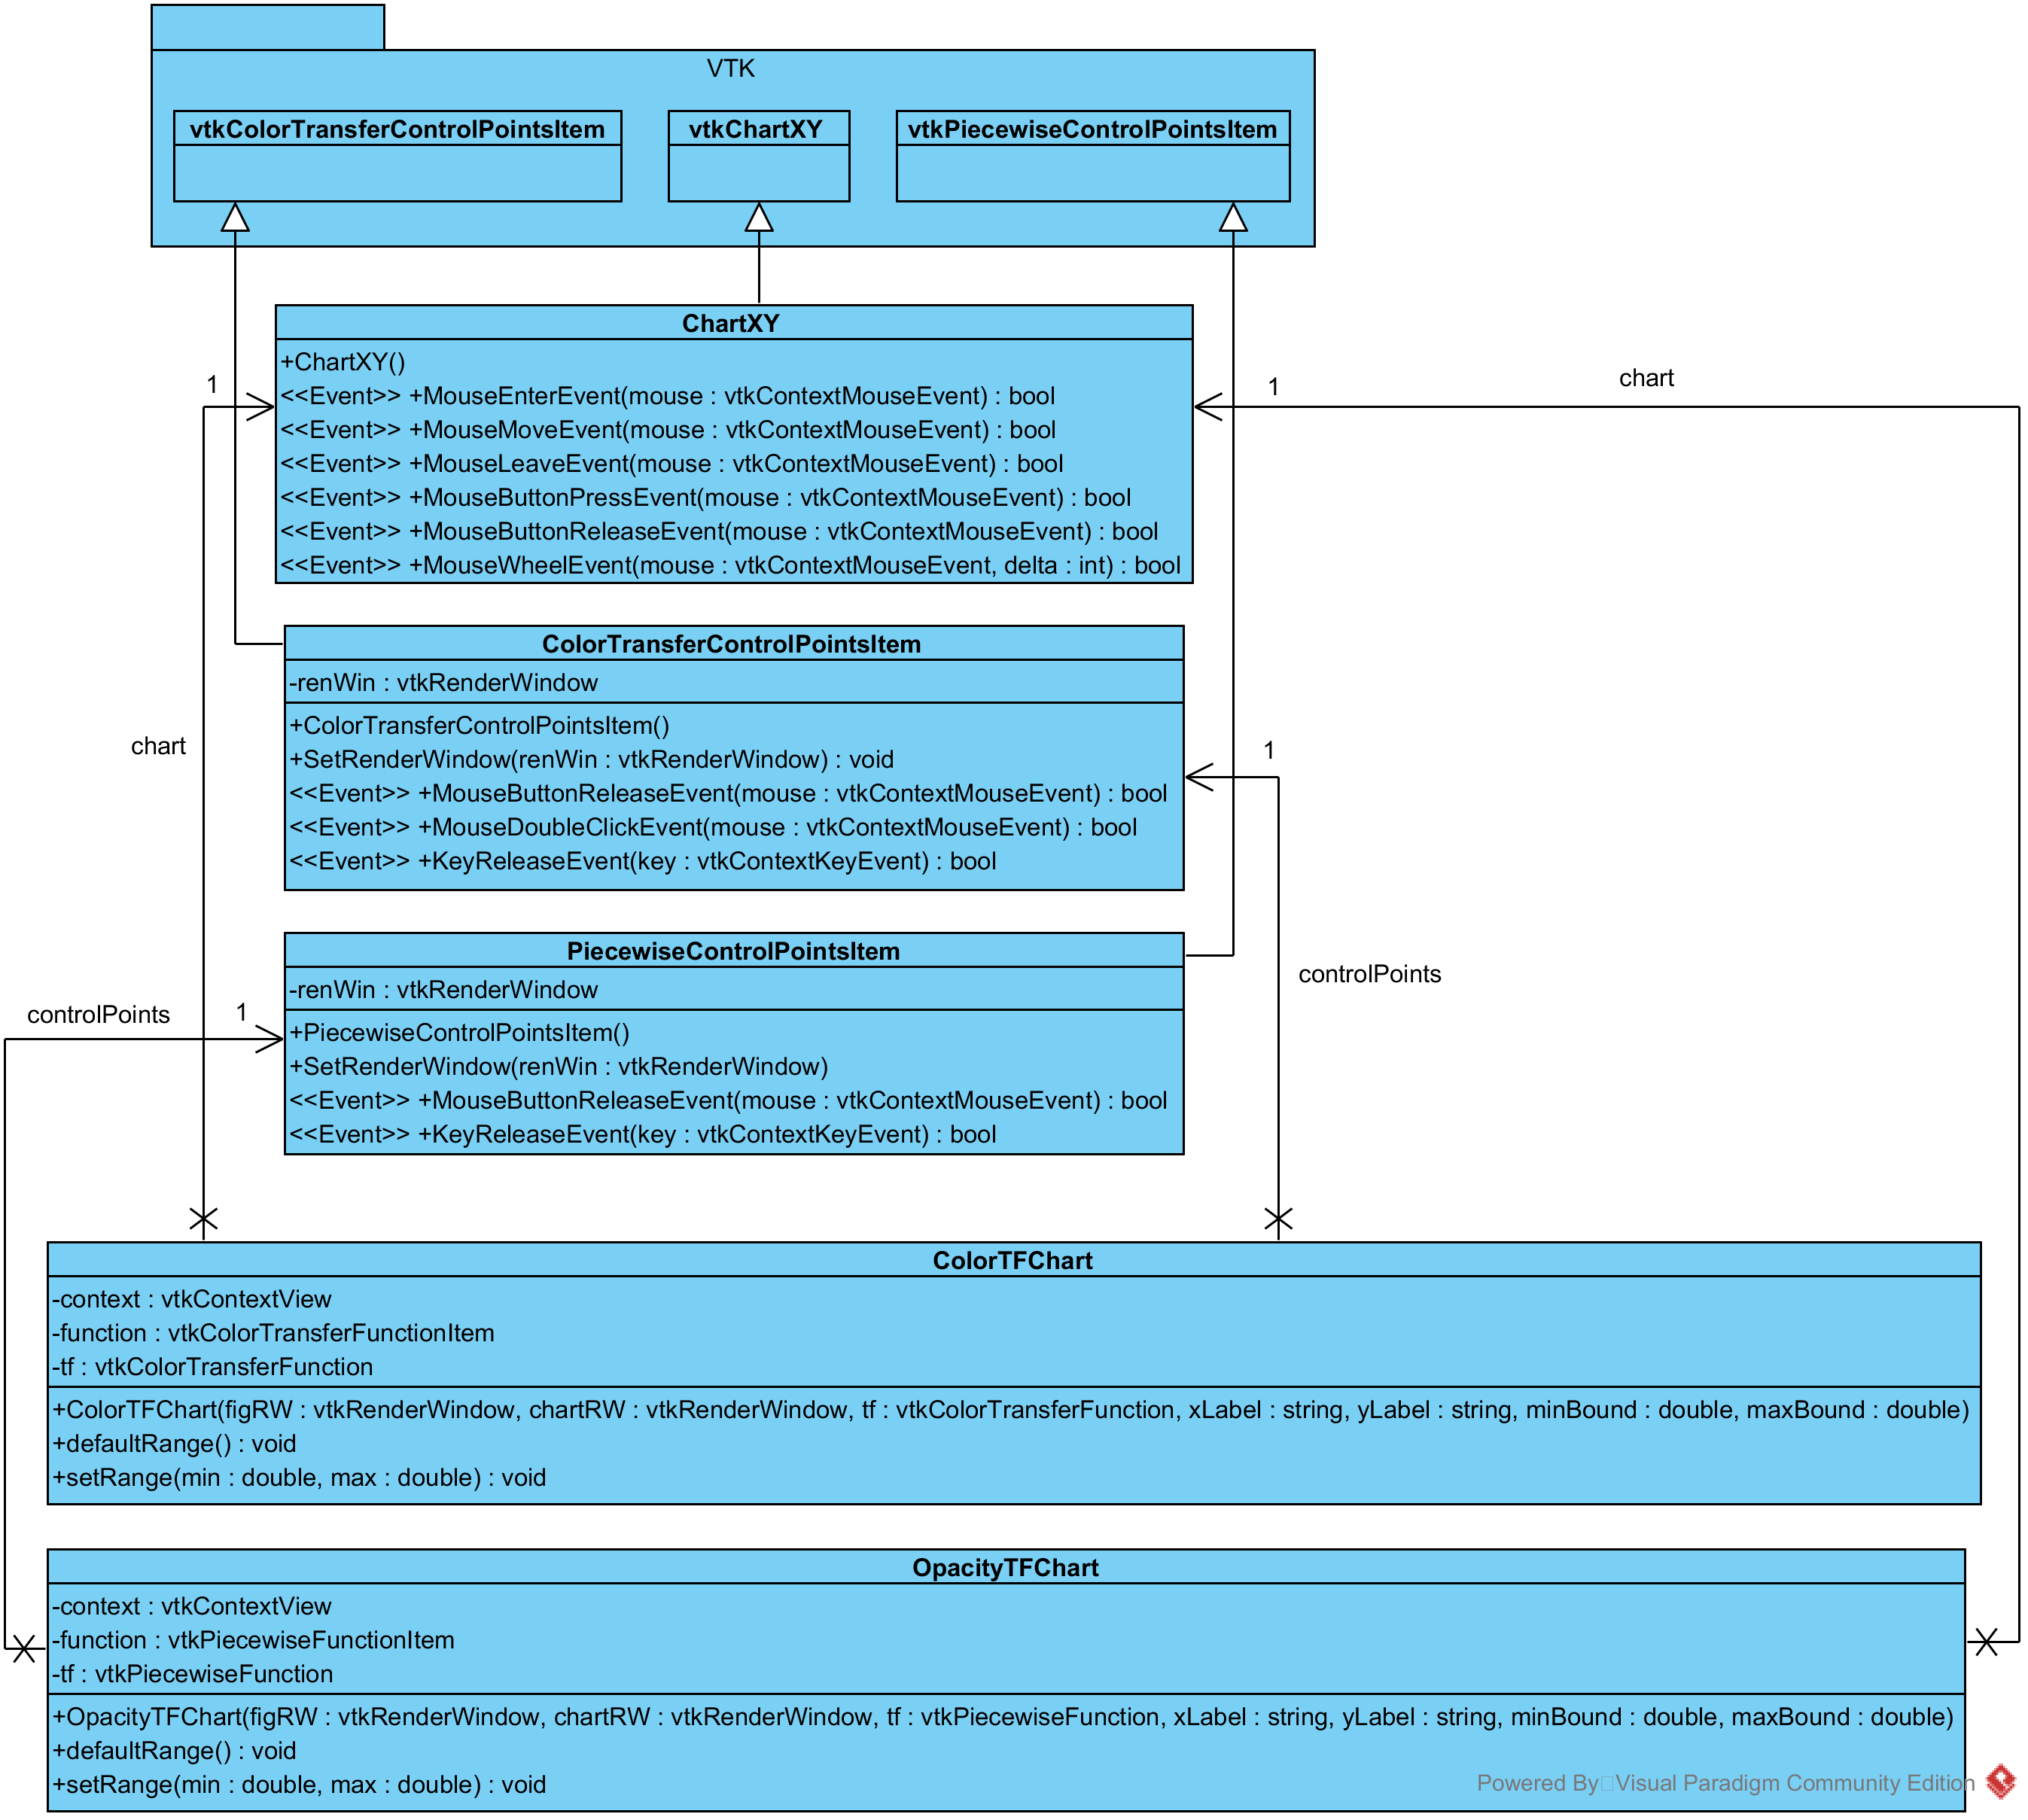
\includegraphics[width=12.5cm]{imagenes/diagramas/charts}
	\caption{Diagrama de clases del paquete \textit{Charts}}
	\label{fig:diagrama_clases_charts}
\end{figure}

\subsection{Paquete Volume}

\begin{figure}[H]
	\centering
	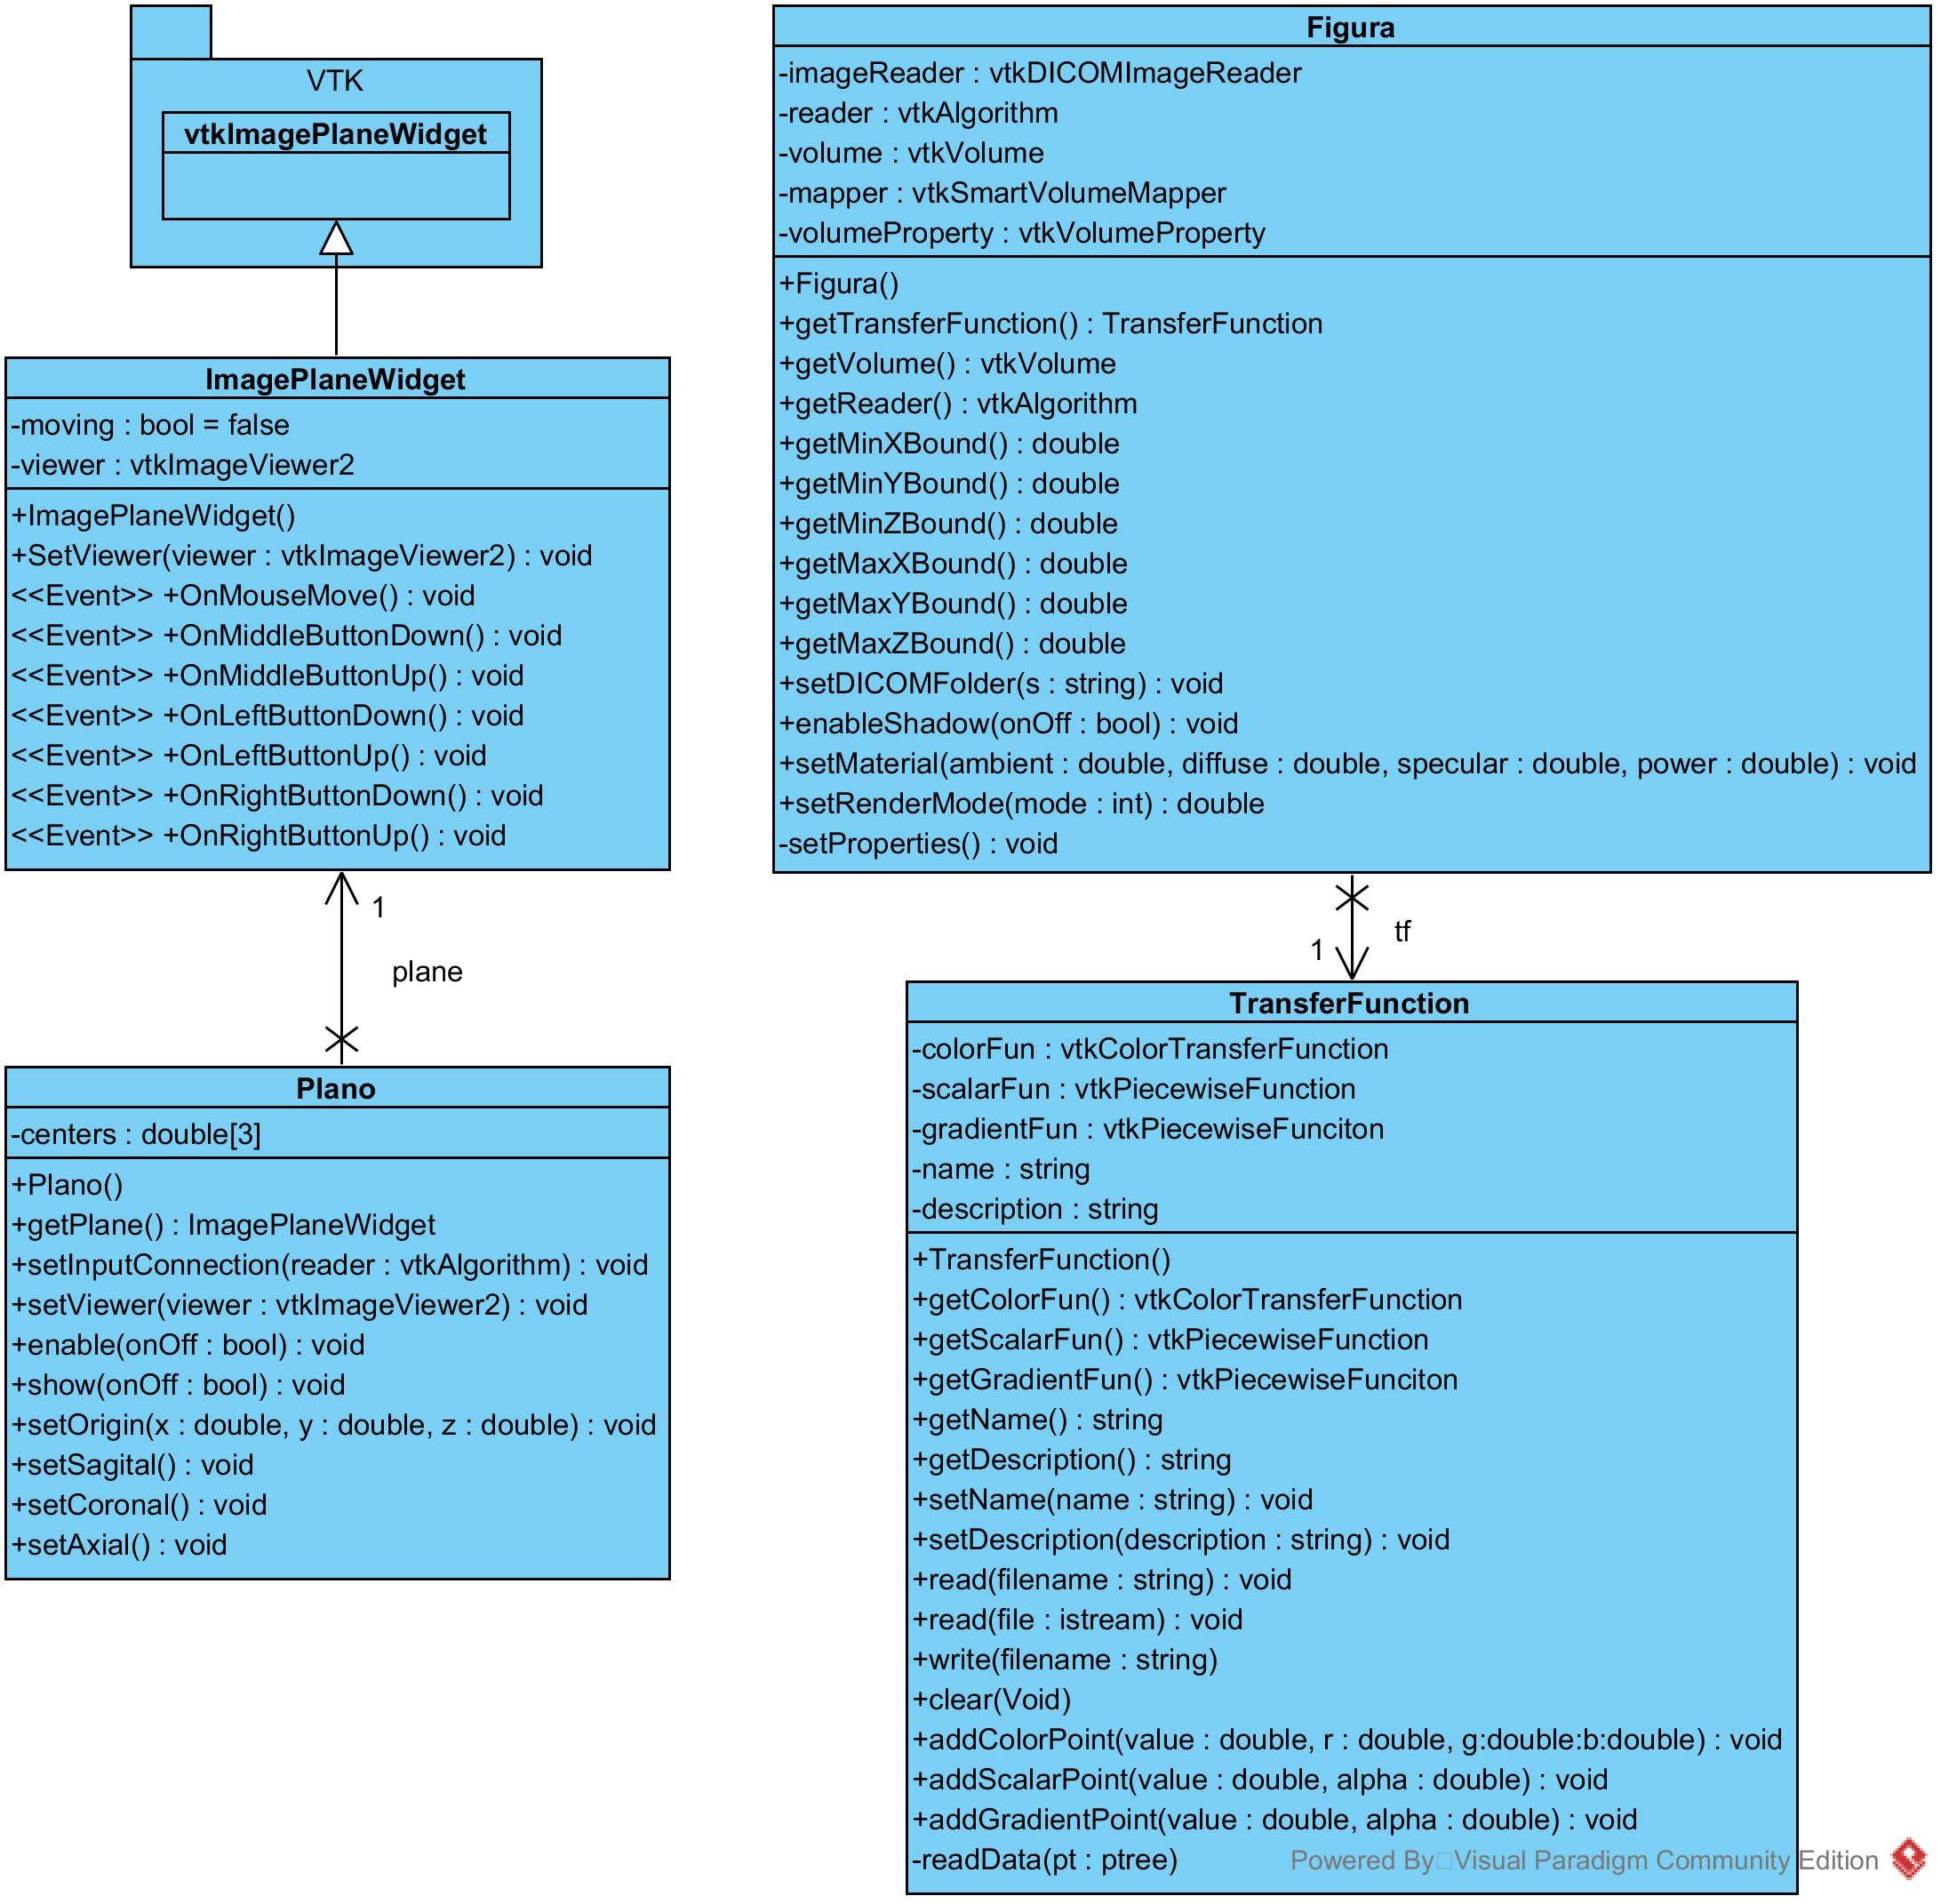
\includegraphics[width=12.5cm]{imagenes/diagramas/volume}
	\caption{Diagrama de clases del paquete \textit{Volume}}
	\label{fig:diagrama_clases_volume}
\end{figure}
% Hablar de los problemas que se han tenido con linux, el cambio de versión ¿por qué y qué problemas dio?
\chapter{Ejemplos}

En este capítulo se presentará el software desde un punto de vista práctica mostrando ejemplos de uso sobre dos esculturas a las que previamente se les hicieron una TC.

Estas esculturas son las de \href{http://patrimonio3d.ugr.es/index.php/granada/escultura/item/18-inmaculada-concepcion}{\textbf{Inmaculada Concepción}} y \href{http://patrimonio3d.ugr.es/index.php/granada/escultura/item/6-san-juan-evangelista}{\textbf{San Juan Evangelista}} \ref{fig:figuras_reales}, ambas patrimonio de la Universidad de Granada y cuyos datos DICOM han sido proporcionados por el proyecto de Portal Virtual de Patrimonio de las Universidades Andaluzas, coordinado por la Universidad de Granada a quién se agradece su cesión.

\begin{figure}[H]
	\centering
	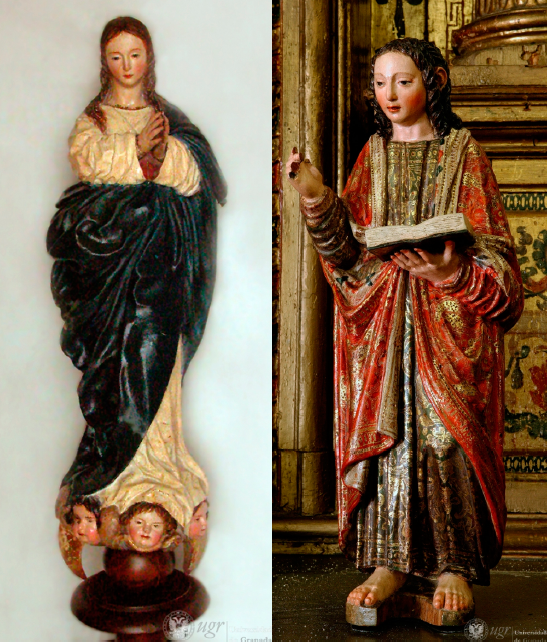
\includegraphics[width=7cm]{imagenes/figuras_reales}
	\caption{Esculturas utilizadas para realizar las pruebas. Inmaculada Concepción (izquierda) y San Juan Evangelista (derecha)}
	\label{fig:figuras_reales}
\end{figure}

\section{Presets}

Se han creado cuatro presets distintos de funciones de transferencias:

\begin{itemize}
	\item \textbf{CT-OnlyWood}: Para mostrar tan solo la madera.
	\item \textbf{CT-OnlyStucco}: Para mostrar tan solo el estuco.
	\item \textbf{CT-OnlyMetal}: Para mostrar el metal (también se ve con mucha transparencia la madera para tener una referencia de dónde se encuentra el metal).
	\item \textbf{CT-WoodSculpture}: Muestra todos los materiales. Es el utilizado al abrir el programa.
\end{itemize}

Gracias a estos se puede ver que la escultura de Inmaculada Concepción (Figura \ref{fig:inmaculada_concepcion}) no tiene objetos metálicos como pueden ser clavos en su interior. Y además, tiene una capa de estuco bastante gruesa sobre todo en el manto, la cara y las manos.

Al contrario, la escultura de San Juan Evangelista (Figura \ref{fig:san_juan_evangelista}) tiene bastante menos estuco y se pueden observar cinco clavos: dos en los pies, dos en la pierna (bastante torcidos) y uno en la cintura.

\begin{figure}[H]
	\centering
	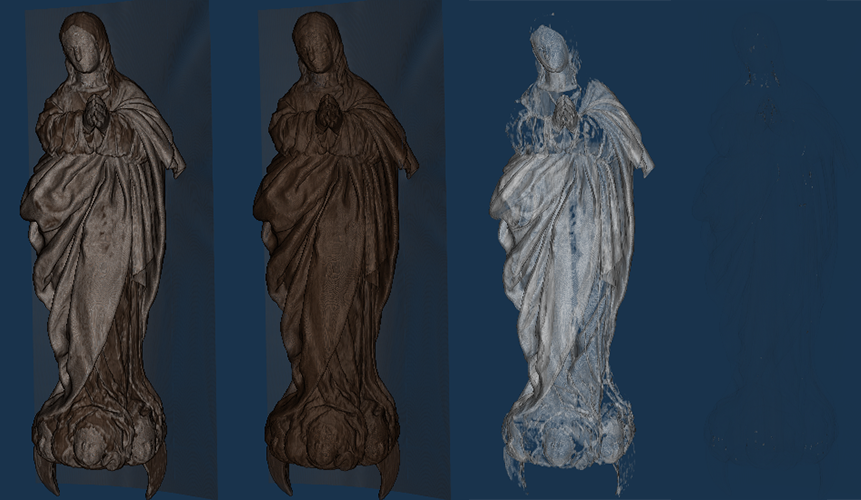
\includegraphics[width=12cm]{imagenes/inmaculada_concepcion}
	\caption{Reconstrucción volumétrica de Inmaculada Concepción usando los cuatro presets proporcionados}
	\label{fig:inmaculada_concepcion}
\end{figure}

\begin{figure}[H]
	\centering
	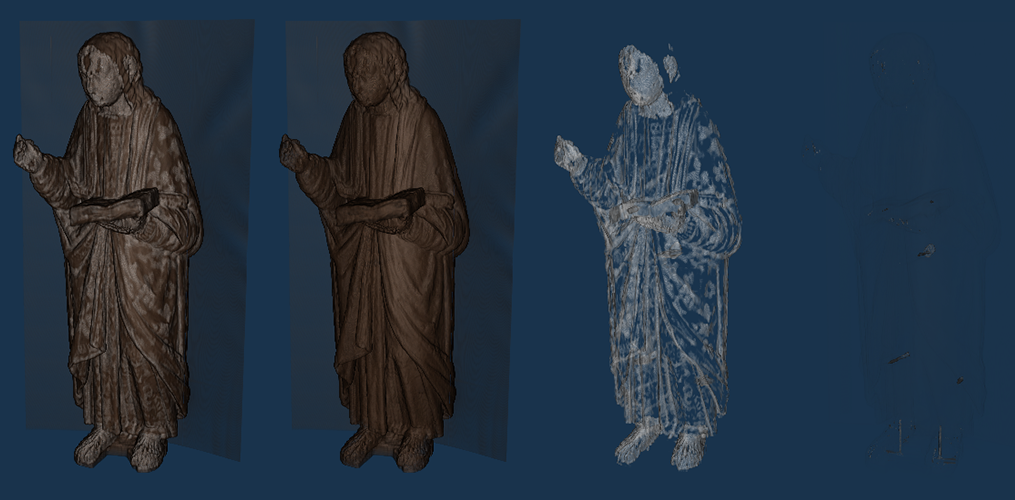
\includegraphics[width=12cm]{imagenes/san_juan_evangelista}
	\caption{Reconstrucción volumétrica de San Juan Evangelista usando los cuatro presets proporcionados}
	\label{fig:san_juan_evangelista}
\end{figure}

Se puede elegir entre estos cuatro presets o cambiar la función de transferencia usando las gráficas (Figura \ref{fig:pestana_funcion_de_transferencia}).

\begin{figure}[H]
	\centering
	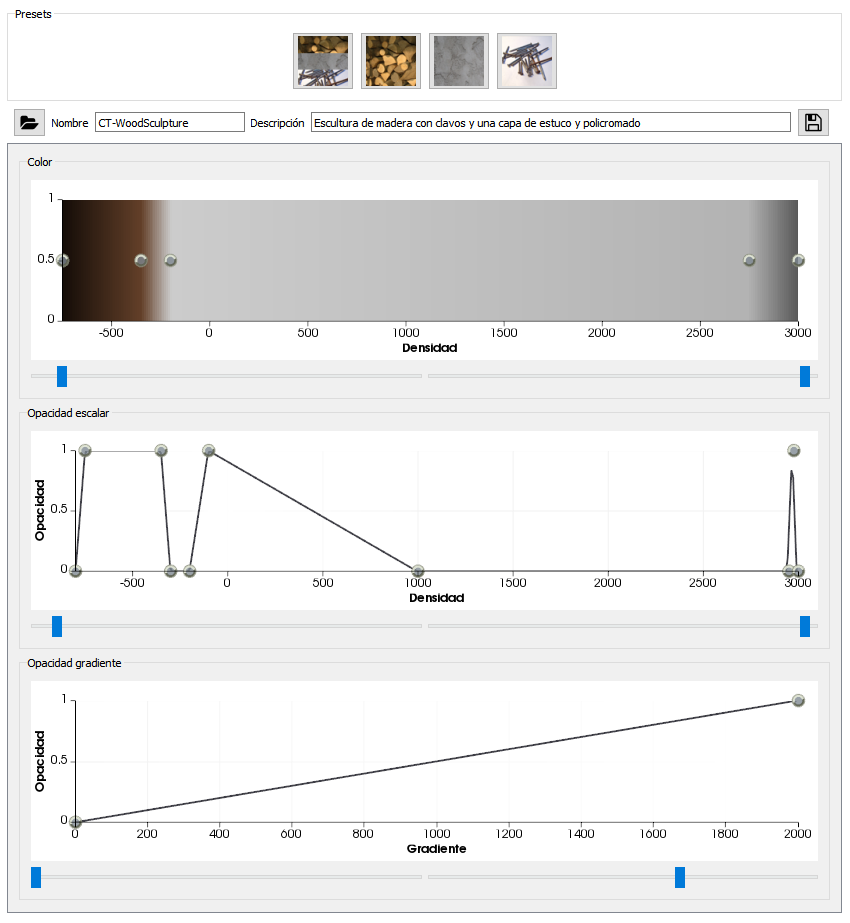
\includegraphics[width=9cm]{imagenes/pestana_funcion_de_transferencia}
	\caption{Pestaña de la GUI donde se puede modificar la función de transferencia}
	\label{fig:pestana_funcion_de_transferencia}
\end{figure}

Desde la GUI (Figura \ref{fig:pestana_funcion_de_transferencia}) además de tener las gráficas y los botones para cambiar de preset se puede importar una función de transferencia o exportar la que se esté usando en ese momento para poder utilizarla en cualquier otro momento o compartirla con otros usuarios.

\section{Plano de corte}

Para interactuar con el plano hay que hacer click derecho sobre éste y moverlo. Para girarlo hay que hacer el click derecho en los bordes de éste. Además desde la GUI (Figura \ref{fig:gui_plano}) se puede cambiar a posiciones por defecto del plano (rojo: sagital, verde: axial y azul: coronal), guardar una imagen del corte y activar o desactivar el plano para que no se muestre en el visor de la reconstrucción volumétrica en 3D.

\begin{figure}[H]
	\centering
	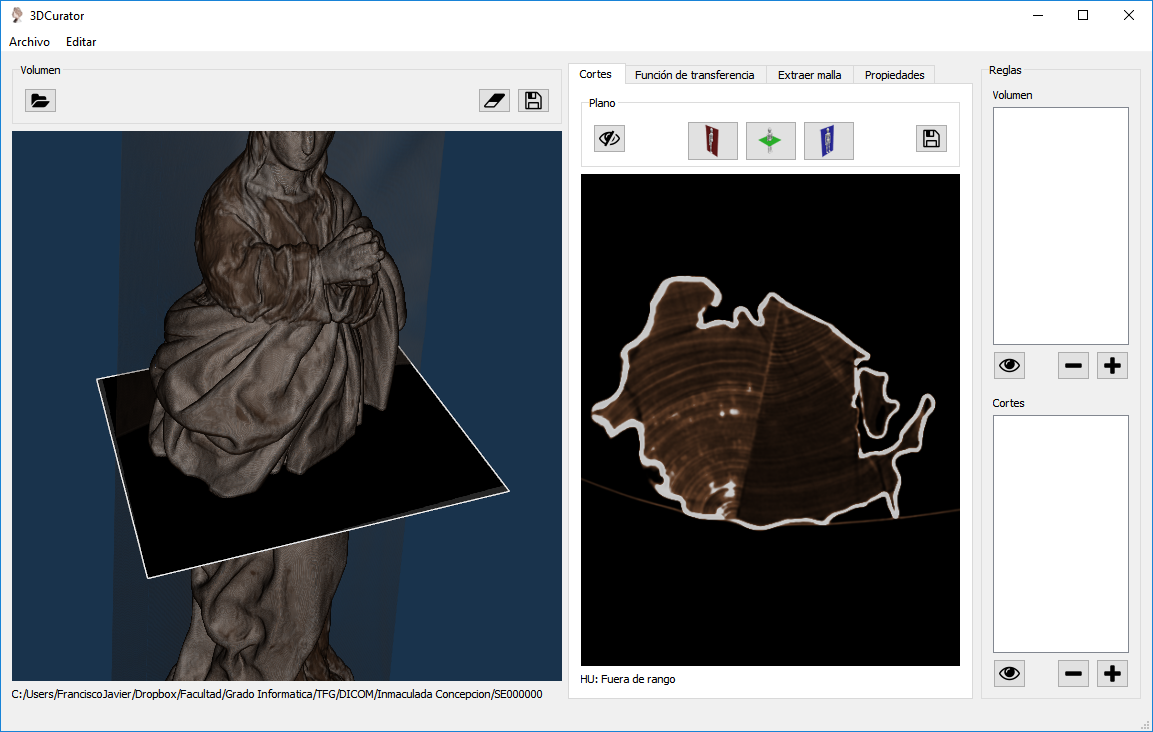
\includegraphics[width=12.5cm]{imagenes/gui_plano}
	\caption{GUI completa con la pestaña del plano activa donde se puede ver el corte que produce el plano oblicuo en la escultura}
	\label{fig:gui_plano}
\end{figure}

La visualización de cortes es tal vez la funcionalidad más útil para un restaurador y es que puede ver el interior de la figura sin tener que dañarla.

En el caso de la Inmaculada Concepción, por ejemplo, en la zona inferior (Figura \ref{fig:corte_inmaculada_concepcion_agujero}) se pueden apreciar hasta cinco piezas de madera distintas: las dos principales base de la escultura,  dos en los laterales y una frontal en la que está la cabeza de un ángel esculpido. Además en este corte se aprecia menos cantidad de estuco que en las zonas donde se encuentra el manto. Se puede observar también el agujero en el centro utilizado para colocar la figura en su soporte, así como los anillos de la madera, útil para determinar la edad de ésta.

\begin{figure}[H]
	\centering
	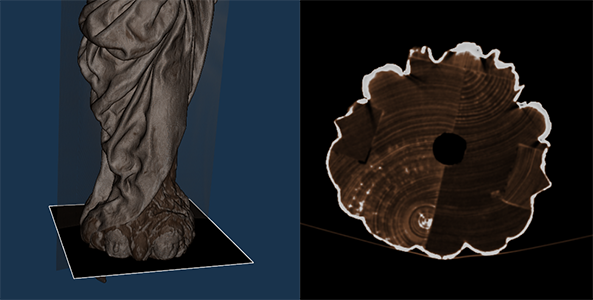
\includegraphics[width=12.5cm]{imagenes/corte_inmaculada_concepcion_agujero}
	\caption{Corte en la zona inferior de la escultura de Inmaculada Concepción}
	\label{fig:corte_inmaculada_concepcion_agujero}
\end{figure}

Examinando la escultura de San Juan Evangelista, también en la zona inferior (Figura \ref{fig:corte_san_juan_evangelista_clavos_pies}) se pueden observar un par de piezas de madera y los dos clavos de los pies.

\begin{figure}[H]
	\centering
	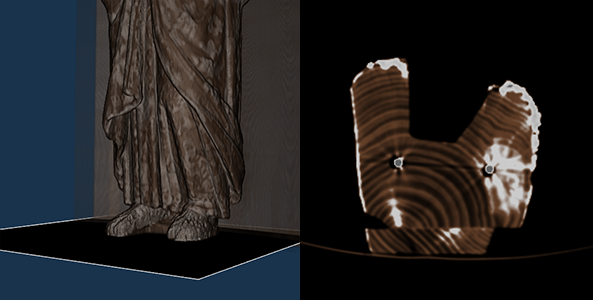
\includegraphics[width=12.5cm]{imagenes/corte_san_juan_evangelista_clavos_pies}
	\caption{Corte en la zona inferior de la escultura de San Juan Evangelista}
	\label{fig:corte_san_juan_evangelista_clavos_pies}
\end{figure}

En el corte anterior se puede ver algo de distorsión producida por el metal, pero donde mejor se puede observar este fenómeno es en el clavo del centro donde parece que hay una zona hueca y otra rellena de estuco, pero realmente estas zonas tienen estos valores por culpa del ruido que produce el clavo durante el escaneo.

\begin{figure}[H]
	\centering
	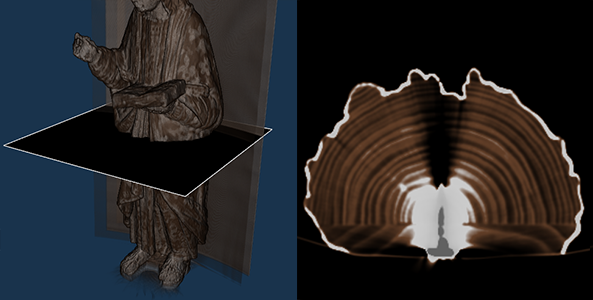
\includegraphics[width=12.5cm]{imagenes/corte_san_juan_evangelista_clavo}
	\caption{Corte en la zona central de la escultura de San Juan Evangelista donde se encuentra el clavo}
	\label{fig:corte_san_juan_evangelista_clavo}
\end{figure}

\section{Reglas}

Una vez obtenidos los cortes, es muy útil tener una herramienta para poder hacer medidas. para así conocer el tamaño de las piezas, agujeros, capas de estuco, clavos...

\begin{figure}[H]
	\centering
	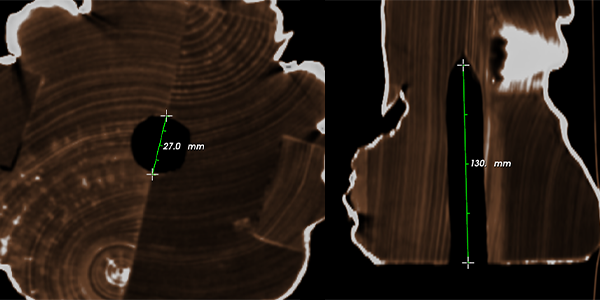
\includegraphics[width=12.5cm]{imagenes/medidas_inmaculada_concepcion_agujero}
	\caption{A la izquierda el diámetro y a la derecha la altura del agujero en el que se introduce el soporte donde se coloca la Inmaculada Concepción}
	\label{fig:medidas_inmaculada_concepcion_agujero}
\end{figure}

Por ejemplo se podrían obtener las dimensiones del agujero de la Inmaculada Concepción (Figura \ref{fig:medidas_inmaculada_concepcion_agujero}).

En el caso de el San Juan Evangelista se podrían medir, por ejemplo, los clavos (Figura\ref{fig:medidas_san_juan_evangelista_clavo}).

\begin{figure}[H]
	\centering
	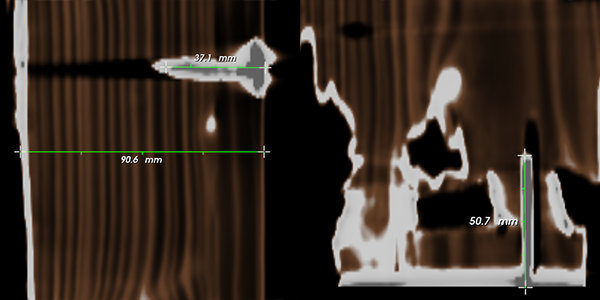
\includegraphics[width=12.5cm]{imagenes/medidas_san_juan_evangelista_clavo}
	\caption{A la izquierda tamaño en profundidad de la pieza y el clavo central y a la derecha tamaño del clavo del pie izquierdo}
	\label{fig:medidas_san_juan_evangelista_clavo}
\end{figure}

\section{Extraer malla}

Para extraer la malla de triángulos el usuario puede elegir entre los presets con los valores de isosuperficie de la madera (que incluye estuco y metal), el estuco (que incluye el metal) y el metal. También puede utilizar un valor personalizado desplazando un \textit{slider} (Figura\ref{fig:pestana_malla}).

\begin{figure}[H]
	\centering
	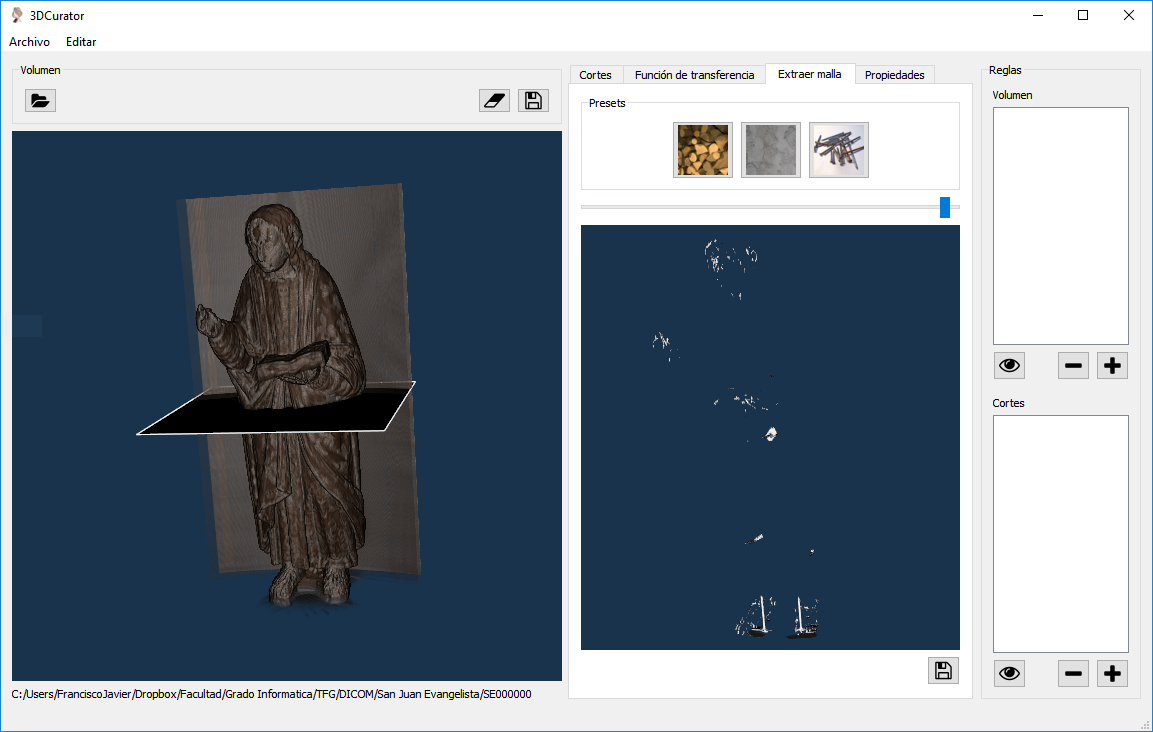
\includegraphics[width=12.5cm]{imagenes/pestana_malla}
	\caption{Pestaña de la GUI para extraer la malla de triángulos}
	\label{fig:pestana_malla}
\end{figure}

Una vez extraída la malla en formato STL se puede usar otro software para trabajar con ella (Figura\ref{fig:malla_clavos_meshlab}).

\begin{figure}[H]
	\centering
	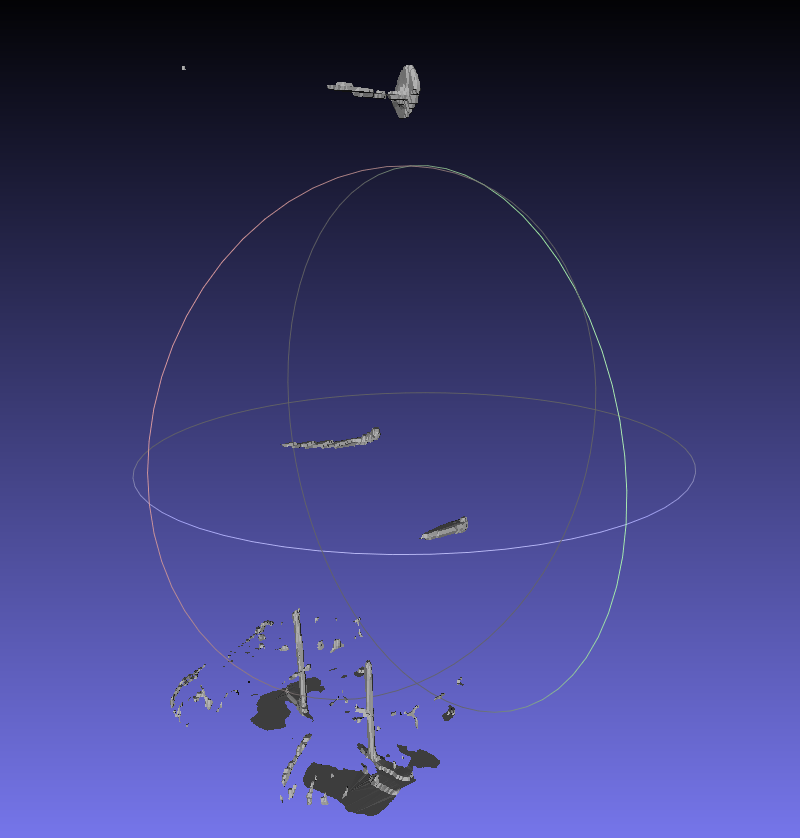
\includegraphics[width=8cm]{imagenes/malla_clavos_meshlab}
	\caption{Malla de los clavos del San Juan Evangelista importada en MeshLab \cite{meshlab}}
	\label{fig:malla_clavos_meshlab}
\end{figure}

\chapter{Conclusiones y trabajos futuros}

En este último capítulo se comentarán las conclusiones a las que se han llegado así como las posibles mejoras en el futuro que se podrían realizar.

\section{Conclusiones}

El uso de la \textbf{TC médica como técnica para examinar las esculturas} de madera policromada en lugar de la radiografía tradicional hemos visto que puede tener muchas ventajas pues puede examinarse el interior de la figura en un espacio 3D sin los problemas de superposición de planos que se daban con la radiografía.

\textbf{Conocer la estructura interna de la escultura es primordial} a la hora de realizar un posterior proceso de conservación y restauración por parte de los restauradores, pero la escasez de herramientas para ello puede ser uno de los motivos por el que esta técnica no ha proliferado todavía.

Durante este proyecto se ha desarrollado un software completo con el que examinar los datos DICOM obtenidos al someter a una escultura a una TC.

Se ha procurado realizar una herramienta \textbf{sencilla de utilizar}, que sea amigable a usuarios que pueden no estar muy habituados al uso de ordenadores para realizar su trabajo. Pero no por ello carente de funcionalidad. Y es que se ha logrado implementar todo lo que se planteó en un principio además de numerosas mejoras.

Por lo que ahora el software cuenta principalmente con la siguiente funcionalidad:

\begin{itemize}
	\item Leer datos DICOM.
	\item Reconstruir volumen a partir de datos DICOM.
	\item Generar y visualizar cortes producidos en la figura por un plano.
	\item Guardar imágenes del volumen y los cortes.
	\item Cambiar de función de transferencia para visualizar unos u otros materiales.
	\item Importar y exportar funciones de transferencia.
	\item Eliminar partes innecesarias del volumen a la hora de la visualización.
	\item Realizar medidas tanto en el volumen como en los cortes.
	\item Generar y exportar una malla de triángulos que contenga un material específico para poder ser posteriormente imprimida.
\end{itemize}

\section{Trabajos futuros}

Las perspectivas futuras del software son altas y pueden realizarse diversas mejoras. En el apartado de nueva funcionalidad:

\begin{itemize}
	\item Además de medir distancias entre dos puntos como se mide ahora se podrían \textbf{medir ángulos} de piezas o definir y \textbf{medir áreas y volúmenes}.
	\item También se podrían \textbf{detectar y definir subvolúmenes de partes} de la escultura con los que trabajar de forma independiente.
	\item Se podría agregar funcionalidad para permitir \textbf{realizar anotaciones} a los restauradores y así no tener que usar lápiz y papel o un software adicional para realizar esta tarea.
	\item Para no tener que escoger la misma carpeta con los datos DICOM cada vez que se importa una escultura, se podría tener una \textbf{base de datos persistente local} donde importar los distintos conjuntos de datos y poder seleccionarlos directamente desde ahí abstrayéndose de dónde están almacenados.
\end{itemize}

También, aprovechando que VTK está disponible para Android (aunque todavía no es estable) se podría migrar la aplicación a \textbf{dispositivos móviles} aprovechando el auge de estos.
%
%\input{capitulos/04_Analisis}
%
%\input{capitulos/05_Diseno}
%
%\input{capitulos/06_Implementacion}
%
%\input{capitulos/07_Pruebas}
%
%\input{capitulos/08_Conclusiones}
%
%%\chapter{Conclusiones y Trabajos Futuros}
%
%
%%\nocite{*}
\bibliography{bibliografia/bibliografia}
\addcontentsline{toc}{chapter}{Bibliografía}
\bibliographystyle{plain}
%
\appendix
\chapter{Manual de usuario}

\section{Requisitos}

\begin{itemize}
	\item Microsoft Windows 7 o superior
	\item Drivers gráficos compatibles con OpenGL 4
	\item 2GB RAM
\end{itemize}

\section{Instalación}

Instalar usando \texttt{3DCurator.msi} siguiendo los siguientes pasos:

\begin{figure}[H]
	\centering
	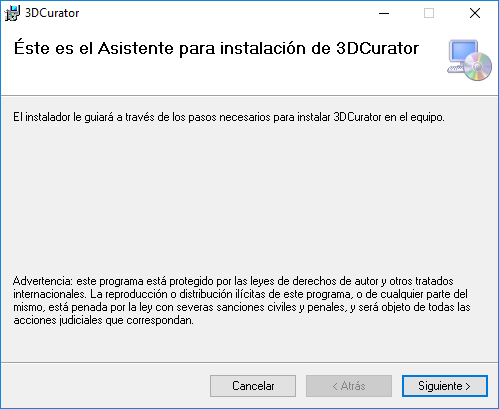
\includegraphics[width=9cm]{imagenes/instalacion_1}
	\caption{Hacer click en Siguiente}
	\label{fig:instalacion_1}
\end{figure}

\begin{figure}[H]
	\centering
	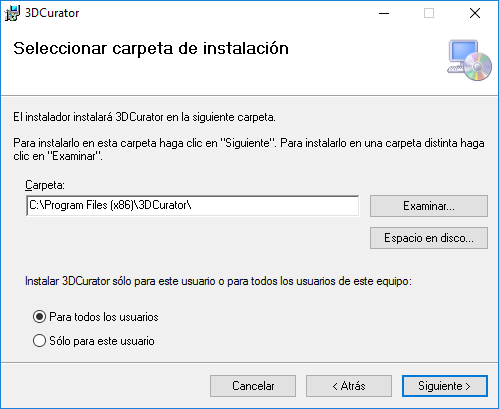
\includegraphics[width=9cm]{imagenes/instalacion_2}
	\caption{Hacer click en Siguiente o cambiar cualquiera de las opciones}
	\label{fig:instalacion_2}
\end{figure}

\begin{figure}[H]
	\centering
	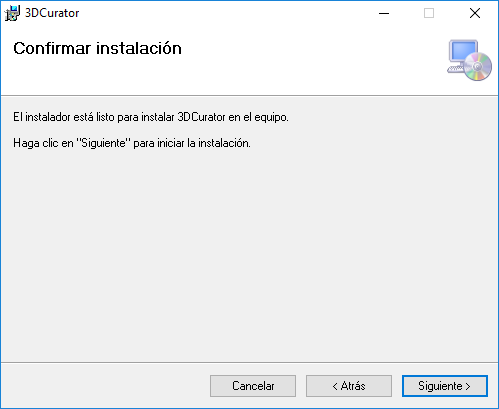
\includegraphics[width=9cm]{imagenes/instalacion_3}
	\caption{Hacer click en Siguiente,  dar permisos de administrador y comenzará a instalarse}
	\label{fig:instalacion_3}
\end{figure}

\begin{figure}[H]
	\centering
	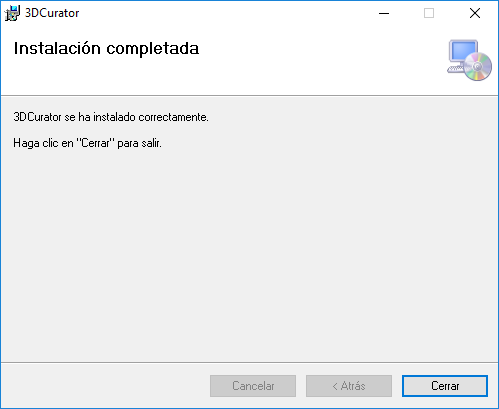
\includegraphics[width=9cm]{imagenes/instalacion_4}
	\caption{Hacer click en Cerrar. Al instalar se habrá creado un acceso directo en el escritorio y en el menú de inicio}
	\label{fig:instalacion_4}
\end{figure}

\section{Capturas de pantalla}

\begin{figure}[H]
	\centering
	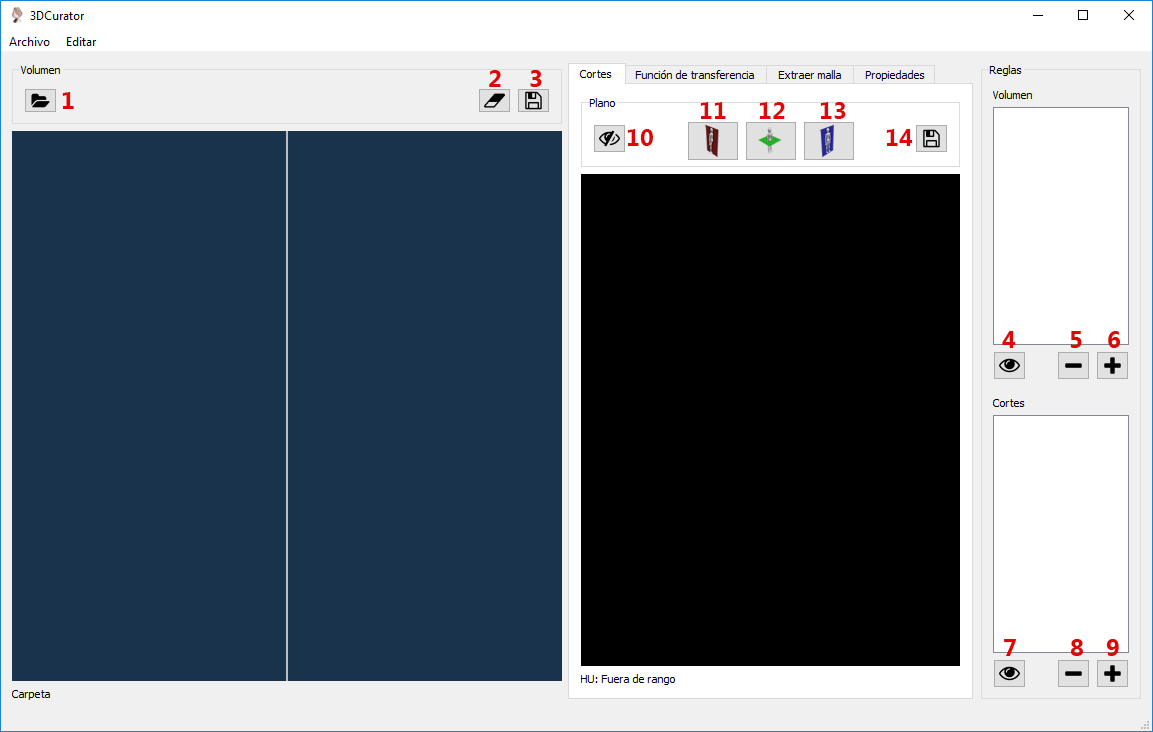
\includegraphics[width=12.5cm]{imagenes/gui_1}
	\caption{Captura de la GUI (Pestaña \textit{Cortes})}
	\label{fig:gui_1}
\end{figure}

\begin{figure}[H]
	\centering
	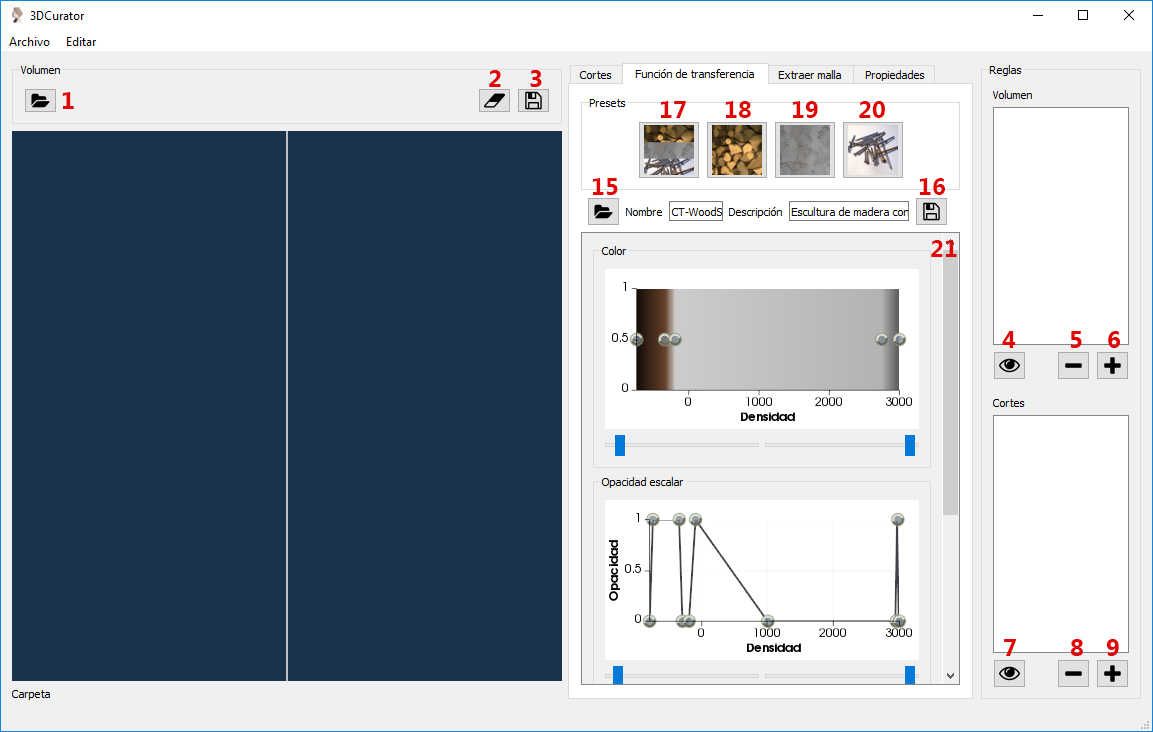
\includegraphics[width=12.5cm]{imagenes/gui_2}
	\caption{Captura de la GUI (Pestaña \textit{Función de transferencia})}
	\label{fig:gui_2}
\end{figure}

\begin{figure}[H]
	\centering
	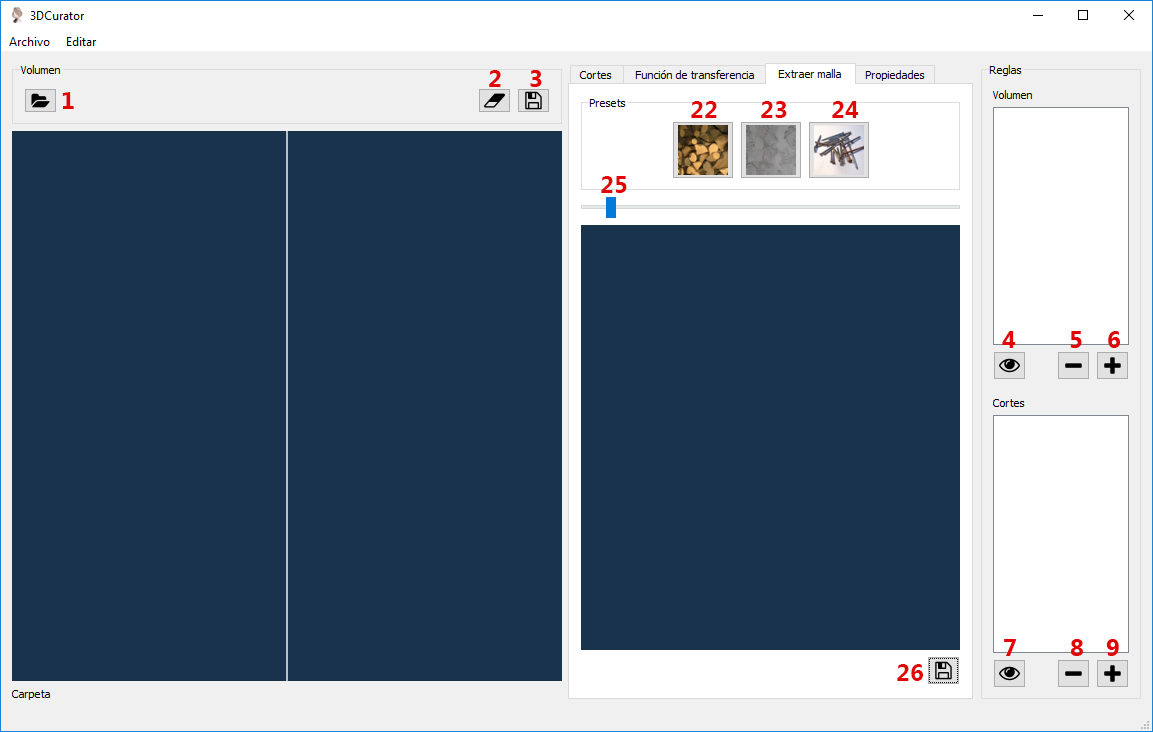
\includegraphics[width=12.5cm]{imagenes/gui_3}
	\caption{Captura de la GUI (Pestaña \textit{Extraer malla})}
	\label{fig:gui_3}
\end{figure}

\begin{figure}[H]
	\centering
	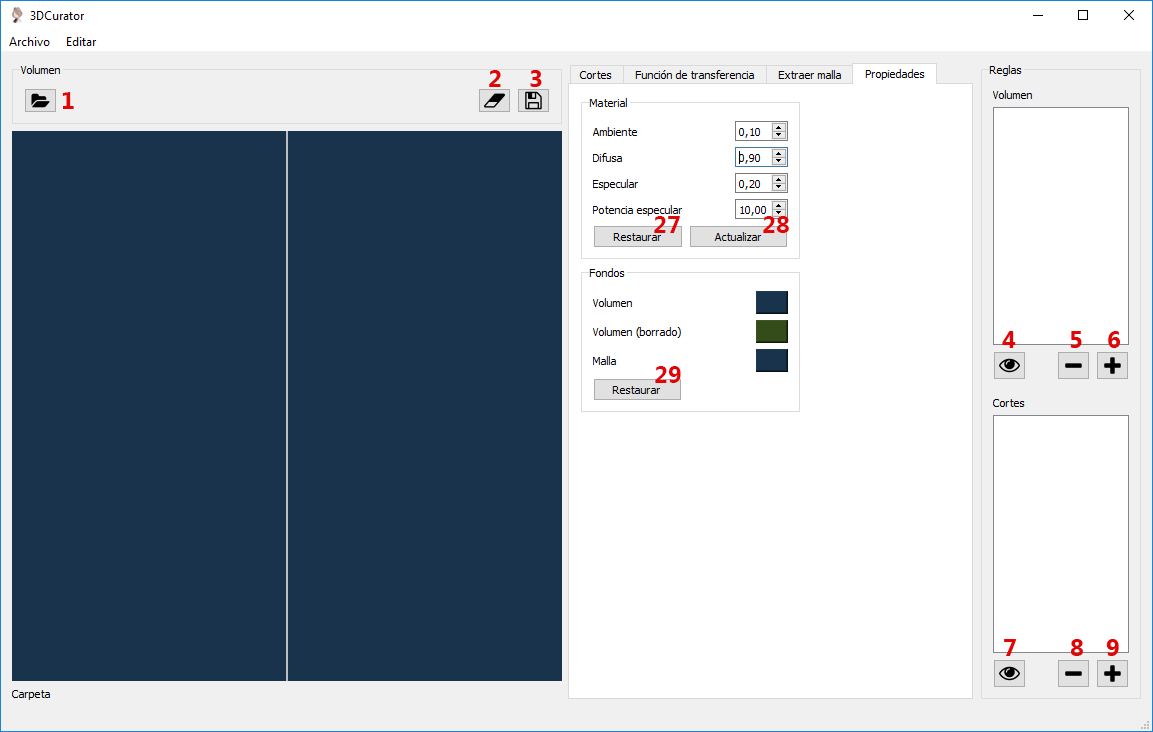
\includegraphics[width=12.5cm]{imagenes/gui_4}
	\caption{Captura de la GUI (Pestaña \textit{Propiedades})}
	\label{fig:gui_4}
\end{figure}

\section{Instrucciones de uso}

\subsection{Abrir directorio DICOM y visualizar datos}

Botón 1, Archivo $ \rangle $ Abrir... o \texttt{Ctrl+O}. Aparecerá una ventana donde se podrá elegir un directorio del sistema. Seleccionar aquel que tenga los archivos DICOM que se quieran importar y pulsar en abrir. Entonces empezará a cargar datos (puede tardar unos segundos). Si hay algún archivo en el directorio que no sea DICOM se mostrará un mensaje de error, pero si ha conseguido cargar el resto se puede continuar con la ejecución del programa sin problema.

Al abrir el archivo DICOM se mostrará la reconstrucción volumétrica en el visor principal, el corte producido con el plano en el visor del plano y la malla en el visor de la malla.

Si se mueve el ratón por el visor del corte abajo de este aparecerá el valor de densidad del pixel sobre el que está el ratón.

\subsubsection{Visor de volumen y malla}

\begin{itemize}
	\item \textbf{Girar cámara}: Click izdo. + arrastrar
	\item \textbf{Mover cámara}: Click central + arrastrar
	\item \textbf{Zoom}: Click dcho. + arrastrar o rueda del ratón
\end{itemize}

\subsubsection{Visor del corte}

\begin{itemize}
	\item \textbf{Mover}: Click central + arrastrar
	\item \textbf{Zoom}: Click dcho. + arrastrar o rueda del ratón
\end{itemize}

\subsection{Eliminar partes de la figura}

Botón 2, Editar $ \rangle $ Borrar partes o \texttt{Ctrl+May+D}. Se cambiará el visor del volumen de color y no se podrá girar la cámara.

Para borrar hacer click en un punto de la isla que se desea borrar. Entendiendo como isla parte que está separada de las demás. El proceso tardará unos segundos dependiendo del tamaño de la parte que se va a borrar. Al borrar se podrá ver el efecto del borrado y confirmar o volver a como estaba antes de borrar.

En ocasiones se necesitará hacer más de un borrado para borrar una isla por completo.

\subsection{Cambiar plano}

\subsubsection{Mostrar/Esconder}

En la pestaña \textit{Cortes} Botón 10, Editar $ \rangle $ Mostrar/Esconder plano o \texttt{Ctrl+May+H}. Esconderá o mostrará el plano en el visor de volumen. No se actualizará la imagen del corte si se ha escondido hasta que no se vuelva a mostrar.

\subsubsection{Posiciones por defecto}

Para colocarlas centradas en un plano anatómico:

\begin{itemize}
	\item \textbf{Sagital}: En la pestaña \textit{Cortes} Botón 11, Editar $ \rangle $ Plano sagital o \texttt{Ctrl+May+S}
	\item \textbf{Axial}: En la pestaña \textit{Cortes} Botón 12, Editar $ \rangle $ Plano axial o \texttt{Ctrl+May+A}
	\item \textbf{Coronal}: En la pestaña \textit{Cortes} Botón 13, Editar $ \rangle $ Plano coronal o \texttt{Ctrl+May+C}
\end{itemize}

\subsubsection{Mover}

El plano se mueve haciendo click derecho sobre éste y arrastrando hacia donde se desea. Para girarlo hacer el click en los extremos del plano.

\subsection{Guardar imagen del volumen}

Botón 3, Archivo $ \rangle $ Exportar figura... o \texttt{Ctrl+F}. Aparecerá una ventana donde se elegirá dónde, con qué nombre y con qué formato guardar la imagen.

\subsection{Guardar imagen del corte}

En la pestaña \textit{Cortes} Botón 14, Archivo $ \rangle $ Exportar corte... o \texttt{Ctrl+F}. Aparecerá una ventana donde se elegirá dónde, con qué nombre y con qué formato guardar la imagen.
 
\subsection{Cambiar color de fondo de visores}

En la pestaña \textit{Propiedades} pulsar sobre el botón coloreado a la derecha del nombre del visor cuyo color de fondo quiera ser cambiado. Aparecerá una ventana para elegir el color.

Si se desean restaurar los colores por defecto, pulsar en el Botón 29.

\subsection{Cambiar material del volumen}

En la pestaña \textit{Propiedades} cambiar los valores de las distintas componentes del material y pulsar en el Botón 28.

Si se desea restaurar el material por defecto, pulsar en el Botón 27.

\subsection{Función de transferencia}

\subsubsection{Cambiar \textit{preset}}

\begin{itemize}
	\item \textbf{Completo}: En la pestaña \textit{Función de transferencia} Botón 11, Editar $ \rangle $ Preset completo o \texttt{F1}
	\item \textbf{Madera}: En la pestaña \textit{Función de transferencia} Botón 12, Editar $ \rangle $ Preset madera o \texttt{F2}
	\item \textbf{Estuco}: En la pestaña \textit{Función de transferencia} Botón 13, Editar $ \rangle $ Preset estuco o \texttt{F3}
	\item \textbf{Metal}: En la pestaña \textit{Función de transferencia} Botón 14, Editar $ \rangle $ Preset metal o \texttt{F4}
\end{itemize}

\subsubsection{Importar}

En la pestaña \textit{Función de transferencia} Botón 15, Herramientas $ \rangle $ Importar preset... o \texttt{Ctrl+May+I}. Aparecerá una ventana donde se podrá escoger el archivo XML con el \textit{preset} que se quiere importar.

En la pestaña \textit{Propiedades} cambiar los valores de las distintas componentes del material y pulsar en el Botón 28.

Si se desea restaurar el material por defecto, pulsar en el Botón 27.

\subsubsection{Exportar}

Editar nombre y descripción en los campos dedicados para ello y, en la pestaña \textit{Función de transferencia} Botón 16, Herramientas $ \rangle $ Exportar preset... o \texttt{Ctrl+May+E}. Aparecerá una ventana donde se podrá escoger el nombre y la ubicación del archivo con el \textit{preset} que se exportará usando la función de transferencia actual.

\subsubsection{Editar}
 
Interactuar con las tres gráficas de la Caja 21 en la pestaña \textit{Función de transferencia}. Se puede cambiar el rango máximo y mínimo que aparece en la gráfica con los \textit{slider} inferiores. Para cambiar los puntos: 

\begin{itemize}
	\item \textbf{Añadir punto}: Click
	\item \textbf{Seleccionar punto}: Click sobre el punto
	\item \textbf{Eliminar punto}: Click central sobre el punto o seleccionar y \texttt{Del} o \texttt{Supr}.
	\item \textbf{Mover punto}: Seleccionar punto y arrastrar
	\item \textbf{Cambiar color}: (Solo en la de color) Doble click. Aparecerá una ventana de selección de color
\end{itemize}

\subsection{Generar malla}

En la pestaña \textit{Extraer malla} usar el Slider 25 para cambiar el valor de isosuperficie. Se generará en unos segundos la malla.

Para elegir entre cualquiera de los \textit{presets}:

\begin{itemize}
	\item \textbf{Madera}: En la pestaña \textit{Extraer malla} Botón 22, Editar $ \rangle $ Malla madera. Incluye los materiales madera, estuco y metal.
	\item \textbf{Estuco}: En la pestaña \textit{Extraer malla} Botón 23, Editar $ \rangle $ Malla estuco. Incluye los materiales estuco y metal.
	\item \textbf{Metal}: En la pestaña \textit{Extraer malla} Botón 24, Editar $ \rangle $ Malla metal. Incluye el material metal.
\end{itemize}

\subsection{Extraer malla}

En la pestaña \textit{Extraer malla} Botón 26, Herramientas $ \rangle $ Extraer malla... o \texttt{Ctrl+May+M}. Aparecerá una ventana donde se elegirá el nombre y la ubicación de la malla que se exportará en formato STL.

\subsection{Realizar medidas}

\subsubsection{Añadir regla}

Según el visor donde se realizará la medida pulsar el botón 6 (visor de volumen) o 9 (visor de cortes). Se hará click derecho en el punto inicial y en el final y aparecerá la medida en milímetros.

\subsubsection{Eliminar regla}

Seleccionar una regla de cualquiera de las cajas de reglas y pulsar en el botón 5 (reglas de volumen) u 8 (reglas de cortes). La regla desaparecerá.

\subsubsection{Mostrar/Esconder regla}

Seleccionar una regla de cualquiera de las cajas de reglas y pulsar en el botón 4 (reglas de volumen) u 7 (reglas de cortes). La regla se mostrará o se esconderá según su estado previo.

\subsubsection{Mover regla}

Click izquierdo en cualquiera de los puntos inicial o final de una regla y arrastrar el ratón.
%%\input{apendices/paper/paper}
%\input{glosario/entradas_glosario}
% \addcontentsline{toc}{chapter}{Glosario}
% \printglossary
%\chapter*{}
%\thispagestyle{empty}

\end{document}
